
\chapter{Inference for categorical data}
\label{inferenceForCategoricalData}

Chapter~\ref{inferenceForCategoricalData} introduces inference in the setting of categorical data. We use these methods to answer questions like the following:
\begin{itemize}
\setlength{\itemsep}{0mm}
\item What proportion of the American public approves of the job the Supreme Court is doing?
\item The Pew Research Center conducted a poll about support for the 2010 health care law, and they used two forms of the survey question. Each respondent was randomly given one of the two questions. What is the difference in the support for respondents under the two question orderings?
\end{itemize}
The methods we learned in previous chapters will continue to be useful in these settings. For example, sample proportions are well characterized by a nearly normal distribution when certain conditions are satisfied, making it possible to employ the usual confidence interval and hypothesis testing tools. In other instances, such as those with contingency tables or when sample size conditions are not met, we will use a different distribution, though the core ideas remain the same.


%__________________
\section{Inference for a single proportion}
\label{singleProportion}

\index{data!Ebola poll|(}

In New York City on October 23rd, 2014, a doctor who had recently been treating Ebola patients in Guinea went to the hospital with a slight fever and was subsequently diagnosed with Ebola. Soon thereafter, an NBC 4 New York/The Wall Street Journal/Marist Poll found that 82\% of New Yorkers favored a ``mandatory 21-day quarantine for anyone who has come in contact with an Ebola patient''.\footnote{\oiRedirect{textbook-maristpoll_ebola_201410}{Poll ID NY141026 on maristpoll.marist.edu}.} This poll included responses of 1,042 New York adults between October 26th and 28th.


\subsection{Identifying when the sample proportion is nearly normal}

A sample proportion can be described as a sample mean. If we represent each ``success'' as a 1 and each ``failure'' as a 0, then the sample proportion is the mean of these numerical outcomes:
\begin{eqnarray*}
\hat{p} = \frac{\ 0 + 1 + 1 + \cdots + 0\ }{1042} = 0.82
\end{eqnarray*}
The distribution of $\hat{p}$ is nearly normal when the distribution of 0's and 1's is not too strongly skewed for the sample size. The most common guideline for sample size and skew when working with proportions is to ensure that we expect to observe a minimum number of successes (1's) and failures (0's), typically at least 10 of each.

\Add{The labels \term{success} and \term{failure} need not mean something positive or negative. These terms are just convenient words frequently used when discussing proportions.}

\begin{termBox}{\tBoxTitle{Conditions for the sampling distribution of $\hat{p}$ being nearly normal}
The sampling distribution for $\hat{p}$, taken from a sample of size $n$ from a population with a true proportion $p$, is nearly normal when
\begin{enumerate}
\item the sample observations are independent and
\item we expected to see at least 10 successes and 10 failures in our sample, i.e. $np\geq10$ and $n(1-p)\geq10$. This is called the \term{success-failure condition}.
\end{enumerate}
If these conditions are met, then the sampling distribution of $\hat{p}$ is nearly normal with mean $p$ and standard error
\index{standard error!single proportion}
\begin{eqnarray}
SE_{\hat{p}} = \sqrt{\frac{\ p(1-p)\ }{n}}
\label{seOfPHat}
\end{eqnarray}}
\end{termBox}\marginpar[\raggedright\vspace{-53mm}

$\hat{p}$\vspace{0mm}\\\footnotesize sample\\proportion\vspace{3mm}\\\normalsize$p$\vspace{0mm}\\\footnotesize population\\proportion]{\raggedright\vspace{-53mm}

$\hat{p}$\vspace{0mm}\\\footnotesize sample\\proportion\vspace{3mm}\\\normalsize$p$\vspace{0mm}\\\footnotesize population\\proportion}

Typically we don't know the true proportion, $p$, so we substitute some value to check conditions and to estimate the standard error. For confidence intervals, usually the sample proportion $\hat{p}$ is used to check the success-failure condition and compute the standard error. For hypothesis tests, typically the null value -- that is, the proportion claimed in the null hypothesis -- is used in place of $p$. Examples are presented for each of these cases in Sections~\ref{confIntForPropSection} and~\ref{htForPropSection}.

\begin{tipBox}{\tipBoxTitle{Reminder on checking independence of observations}
If data come from a simple random sample and consist of less than 10\% of the population, then the independence assumption is reasonable. Alternatively, if the data come from a random process, we must evaluate the independence condition more carefully.}
\end{tipBox}


\subsection{Confidence intervals for a proportion}
\label{confIntForPropSection}

\index{point estimate!single proportion}

We may want a confidence interval for the proportion of New York adults who favored a mandatory quarantine of anyone who had been in contact with an Ebola patient. Our point estimate, based on a sample of size $n = 1042$, is $\hat{p} = 0.82$. We would like to use the general confidence interval formula from Section~\ref{aFrameworkForInference}. However, first we must verify the sampling distribution of $\hat{p}$ is nearly normal and calculate the standard error of $\hat{p}$.
\begin{description}
\item[Observations are independent.] The poll is based on a simple random sample and consists of fewer than 10\% of the New York adult population, which verifies independence.
\item[Success-failure condition.] The sample size must also be sufficiently large, which is checked using the \hiddenterm{success-failure condition}. There were $1042 \times \hat{p} \approx 854$ ``successes'' and $1042 \times (1 - \hat{p}) \approx 188$ ``failures'' in the sample, both easily greater than~10.
\end{description}
With the conditions met, we are assured that the sampling distribution of $\hat{p}$ is nearly normal. Next, a standard error for $\hat{p}$ is needed, and then we can employ the usual method to construct a confidence interval.

\begin{exercise} \label{seOfPropOfAmericansJobApprovalOfSupremeCourt}
Estimate the standard error of $\hat{p}=0.44$ using Equation~\eqref{seOfPHat}. Because $p$ is unknown and the standard error is for a confidence interval, we use $\hat{p}$ in place of $p$ in the formula.\footnote{$SE = \sqrt{\frac{p(1-p)}{n}} \approx \sqrt{\frac{0.82 (1 - 0.82)}{1042}} = 0.012$.}
\end{exercise}

\begin{example}{Construct a 95\% confidence interval for $p$, the proportion of New York adults who supported a quarantine for anyone who has come into contact with an Ebola patient.}
Using the standard error $SE = 0.012$ from Guided Practice~\ref{seOfPropOfAmericansJobApprovalOfSupremeCourt}, the point estimate 0.82, and $z^{\star} = 1.96$ for a 95\% confidence interval, the confidence interval may be computed as
\begin{eqnarray*}
\text{point estimate} \ \pm\ z^{\star}SE \quad\to\quad 0.82 \ \pm\ 1.96\times 0.012 \quad\to\quad (0.796, 0.844)
\end{eqnarray*}
We are 95\% confident that the true proportion of New York adults in October 2014 who supported a quarantine for anyone who has come into contact with an Ebola patient was between 0.796 and 0.844.

\index{data!Ebola poll|)}

\end{example}

Notice that since the poll was around the time where a doctor in New York had come down with Ebola, the results may not be as applicable today as they were at the time the poll was taken. This highlights an important detail about polls: they provide data about public opinion at a single point in time.

\begin{termBox}{\tBoxTitle[]{Constructing a confidence interval for a proportion}\vspace{-1mm}
\begin{itemize}
\setlength{\itemsep}{0mm}
\item Verify the observations are independent and also verify the success-failure condition using $\hat{p}$ and $n$.
\item If the conditions are met, the sampling distribution of $\hat{p}$ may be well-approximated by the normal model.
\item Construct the standard error using $\hat{p}$ in place of $p$ and apply the general confidence interval formula.\vspace{1mm}
\end{itemize}}
\end{termBox}


\subsection{Hypothesis testing for a proportion}
\label{htForPropSection}

To apply the normal distribution framework in the context of a hypothesis test for a proportion, the independence and success-failure conditions must be satisfied. In a hypothesis test, the success-failure condition is checked using the null proportion: we verify $np_0$ and $n(1-p_0)$ are at least 10, where $p_0$ is the null value.

\index{data!nuclear arms reduction|(}

\begin{exercise}
Do a majority of American support nuclear arms reduction? Set up a one-sided hypothesis test to evaluate this question.\footnote{$H_0: p = 0.50$. $H_A: p > 0.50$.}
\end{exercise}

\begin{example}{A simple random sample of 1,028 US adults in March 2013 found that 56\% support nuclear arms reduction.\footnote{\oiRedirect{textbook-nuclear_arms_reduction_201303}{www.gallup.com/poll/161198/favor-russian-nuclear-arms-reductions.aspx}} Does this provide convincing evidence that a majority of Americans supported nuclear arms reduction at the 5\% significance level?} \label{NuclearArmsInferenceExample}
The poll was of a simple random sample that includes fewer than 10\% of US adults, meaning the observations are independent. In a one-proportion hypothesis test, the success-failure condition is checked using the null proportion, which is $p_0 = 0.5$ in this context: $n p_0 = n (1 - p_0) = 1028 \times 0.5 = 514 > 10$. With these conditions verified, the normal model may be applied to $\hat{p}$.

Next the standard error can be computed. The null value $p_0$ is used again here, because this is a hypothesis test for a single proportion.
\begin{align*}
SE = \sqrt{\frac{p_0 (1 - p_0)}{n}} = \sqrt{\frac{0.5 (1 - 0.5)}{1028}} = 0.016
\end{align*}
A picture of the normal model is shown in Figure~\ref{nuclearArmsReductionPValue} with the p-value represented by the shaded region. Based on the normal model, the test statistic can be computed as the Z score of the point estimate:
\begin{align*}
Z = \frac{\text{point estimate} - \text{null value}}{SE} = \frac{0.56 - 0.50}{0.016} = 3.75
\end{align*}
The upper tail area, representing the p-value, is about 0.00009. Because the p-value is smaller than 0.05, we reject $H_0$. The poll provides convincing evidence that a majority of Americans supported nuclear arms reduction efforts in March 2013.
\end{example}

\begin{figure}[h]
\centering
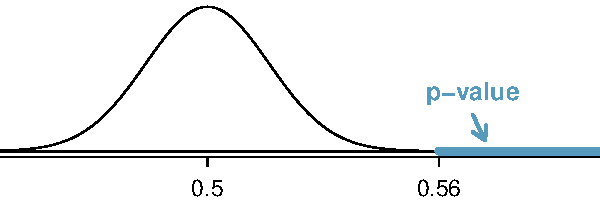
\includegraphics[width=0.6\textwidth]{ch_inference_for_props/figures/nuclearArmsReduction/nuclearArmsReductionPValue}
\caption{Sampling distribution of the sample proportion if the null hypothesis is true for Example~\ref{NuclearArmsInferenceExample}. The area representing the p-value is too small to be visible.}
\label{nuclearArmsReductionPValue}
\end{figure}

\begin{termBox}{\tBoxTitle{Hypothesis test for a proportion}
Set up hypotheses and verify the conditions using the null value, $p_0$, to ensure $\hat{p}$ is nearly normal under $H_0$. If the conditions hold, construct the standard error, again using $p_0$, and show the p-value in a drawing. Lastly, compute the p-value and evaluate the hypotheses.}
\end{termBox}

\index{data!nuclear arms reduction|)}

\CalculatorVideos{confidence intervals and hypothesis tests for a single proportion}


\subsection{Choosing a sample size when estimating a proportion}

\index{margin of error|(}

When collecting data, we choose a sample size suitable for the purpose of the study. Often times this means choosing a sample size large enough that the \term{margin of error} -- which is the part we add and subtract from the point estimate in a confidence interval -- is sufficiently small that the sample is useful. More explicitly, our task is to find a sample size $n$ so that the sample proportion is within some margin of error $m$ of the actual proportion with a certain level of confidence.

% For example, the margin of error for a point estimate using 95\% confidence can be written as $1.96\times SE$. We set up a general equation to represent the problem:
%\begin{align*}
%ME = z^{\star}SE \leq m
%\end{align*}
%where $ME$ represented the actual margin of error and $z^{\star}$ was chosen to correspond to the confidence level. The standard error formula is specified to correspond to the particular setting. For instance, in the case of means, the standard error was given as $\sigma / \sqrt{n}$. In the case of a single proportion, we use $\sqrt{p(1-p) / n\ }$ for the standard error.

\begin{example}{A university newspaper is conducting a survey to determine what fraction of students support a \$200 per year increase in fees to pay for a new football stadium. How big of a sample is required to ensure the margin of error is smaller than 0.04 using a 95\% confidence level?}
The margin of error for a sample proportion is
\begin{align*}
z^{\star} \sqrt{\frac{p (1 - p)}{n}}
\end{align*}
Our goal is to find the smallest sample size $n$ so that this margin of error is smaller than $m=0.04$. For a 95\% confidence level, the value $z^{\star}$ corresponds to 1.96:
\begin{align*}
1.96\times \sqrt{\frac{p(1-p)}{n}} \ < \ 0.04
\end{align*}
There are two unknowns in the equation: $p$ and $n$. If we have an estimate of $p$, perhaps from a similar survey, we could enter in that value and solve for $n$. If we have no such estimate, we must use some other value for $p$. It turns out that the margin of error is largest when $p$ is 0.5, so we typically use this \emph{worst case value} if no estimate of the proportion is available:
\begin{align*}
	1.96\times \sqrt{\frac{0.5(1-0.5)}{n}} &\ < \ 0.04 \\
	1.96^2\times \frac{0.5(1-0.5)}{n} &\ < \ 0.04^2 \\
	1.96^2\times \frac{0.5(1-0.5)}{0.04^2} &\ < \ n \\
	600.25 &\ < \  n
\end{align*}
We would need over 600.25 participants, which means we need 601 participants or more, to ensure the sample proportion is within 0.04 of the true proportion with 95\% confidence.
\end{example}

When an estimate of the proportion is available, we use it in place of the worst case proportion value,~0.5.

\begin{example}{A manager is about to oversee the mass production of a new tire model in her factory, and she would like to estimate what proportion of these tires will be rejected through quality control. The quality control team has monitored the last three tire models produced by the factory, failing 1.7\% of tires in the first model, 6.2\% of the second model, and 1.3\% of the third model. The manager would like to examine enough tires to estimate the failure rate of the new tire model to within about 2\% with a 90\% confidence level.
\begin{enumerate}
\setlength{\itemsep}{0mm}
\item[(a)] There are three different failure rates to choose from. Perform the sample size computation for each separately, and identify three sample sizes to consider.
\item[(b)] The sample sizes vary widely. Which of the three would you suggest using? What would influence your choice?
\end{enumerate}}
(a)~For a 90\% confidence interval, $z^{\star} = 1.65$, and since an estimate of the proportion 0.017 is available, we'll use it in the margin of error formula: %use theFor the 1.7\% estimate of $p$, we estimate the appropriate sample size as follows:
\begin{align*}
1.65\times \sqrt{\frac{0.017(1-0.017)}{n}} &\ < \ 0.02 \\
113.7 &\ < \ n
\end{align*}
For sample size calculations, we always round up, so the first tire model suggests 114 tires would be sufficient.

A similar computation can be accomplished using 0.062 and 0.013 for $p$, and you should verify that using these proportions results in minimum sample sizes of 396 and~88 tires, respectively.

(b) We could examine which of the old models is most like the new model, then choose the corresponding sample size. Or if two of the previous estimates are based on small samples while the other is based on a larger sample, we should consider the value corresponding to the larger sample. There is no one clearly correct approach here. Can you think of other reasonable approaches?
\end{example}

\index{data!Congress approval rating|(}

\begin{exercise}
A recent estimate of Congress' approval rating was 19\%.\footnote{\oiRedirect{textbook-congress_at_19_in_May2015}{www.gallup.com/poll/183128/five-months-gop-congress-approval-remains-low.aspx}} What sample size does this estimate suggest we should use for a margin of error of 0.04 with 95\% confidence?\footnote{We complete the same computations as before, except now we use $0.19$ instead of $0.5$ for $p$:
\begin{align*}
1.96\times \sqrt{\frac{p(1-p)}{n}} \approx
1.96\times \sqrt{\frac{0.19(1-0.19)}{n}} &\leq 0.04 \qquad\to\qquad n \geq 369.5
\end{align*}
A sample size of 370 or more would be reasonable. (Reminder: always round up for sample size calculations!)}

\index{data!Congress approval rating|)}
\index{margin of error|)}

\end{exercise}


%__________________
\section{Difference of two proportions}
\label{differenceOfTwoProportions}

We would like to make conclusions about the difference in two population proportions: $p_1 - p_2$. We consider three examples. In the first, we compare the approval of the 2010 healthcare law under two different question phrasings. In the second application, a company weighs whether they should switch to a higher quality parts manufacturer. In the last example, we examine the cancer risk to dogs from the use of yard herbicides.

In our investigations, we first identify a reasonable point estimate of $p_1 - p_2$ based on the sample. You may have already guessed its form: $\hat{p}_1 - \hat{p}_2$\index{point estimate!difference of proportions}. Next, in each example we verify that the point estimate follows the normal model by checking certain conditions. Finally, we compute the estimate's standard error and apply our inferential framework.


\subsection{Sample distribution of the difference of two proportions}

We must check two conditions before applying the normal model to $\hat{p}_1 - \hat{p}_2$. First, the sampling distribution for each sample proportion must be nearly normal, and secondly, the samples must be independent. Under these two conditions, the sampling distribution of $\hat{p}_1 - \hat{p}_2$ may be well approximated using the normal model.

\begin{termBox}{\tBoxTitle{Conditions for the sampling distribution of $\hat{p}_1 - \hat{p}_2$ to be normal}
The difference $\hat{p}_1 - \hat{p}_2$ tends to follow a normal model when
\begin{itemize}
\setlength{\itemsep}{0mm}
\item each proportion separately follows a normal model, and
\item the two samples are independent of each other.
\end{itemize}
The standard error of the difference in sample proportions is
\index{standard error!difference in proportions}
\begin{eqnarray}
SE_{\hat{p}_1 - \hat{p}_2}
	= \sqrt{SE_{\hat{p}_1}^2 + SE_{\hat{p}_2}^2}
	= \sqrt{\frac{p_1(1-p_1)}{n_1} + \frac{p_2(1-p_2)}{n_2}}
\label{seForDiffOfProp}
\end{eqnarray}
where $p_1$ and $p_2$ represent the population proportions, and $n_1$ and $n_2$ represent the sample sizes.}
\end{termBox}

For the difference in two means, the standard error formula took the following form:
\begin{eqnarray*}
SE_{\bar{x}_{1} - \bar{x}_{2}} = \sqrt{SE_{\bar{x}_1}^2 + SE_{\bar{x}_2}^2}
\end{eqnarray*}
The standard error for the difference in two proportions takes a similar form. The reasons behind this similarity are rooted in the probability theory of Section~\ref{randomVariablesSection}, which is described for this context in Guided Practice~\vref{derivingSEForDiffOfTwoMeansExercise}.


\subsection{Confidence intervals for $p_1 -p_2$}

In the setting of confidence intervals for a difference of two proportions, the two sample proportions are used to verify the success-failure condition and also compute the standard error, just as was the case with a single proportion.

\begin{example}{The way a question is phrased can influence a person's response. For example, Pew Research Center conducted a survey with the following question:\footnote{\oiRedirect{textbook-health_care_bill_2012}{www.people-press.org/2012/03/26/public-remains-split-on-health-care-bill-opposed-to-mandate}{www.people-press.org/2012/03/26/public-remains-split-on-health-care-bill-opposed-to-mandate/}. Sample sizes for each polling group are approximate.}
\begin{quote}
As you may know, by 2014 nearly all Americans will be required to have health insurance. [People who do not buy insurance will pay a penalty] while [People who cannot afford it will receive financial help from the government]. Do you approve or disapprove of this policy?
\end{quote}
\index{data!health care|(}For each randomly sampled respondent, the statements in brackets were randomized: either they were kept in the order given above, or the two statements were reversed. Table~\ref{pewPollResultsForRandomizedStatementOrdering} shows the results of this experiment. Create and interpret a 90\% confidence interval of the difference in approval.}

\begin{table}[t]
\centering
\begin{tabular}{p{50mm}c p{13mm}p{14mm}p{16.5mm}c}
	&\ & Sample size ($n_i$) & Approve law (\%)	& Disapprove law (\%)	& Other \\
\hline
``people who cannot afford it will receive financial help from the government'' is given second \vspace{2.5mm}
	& & 771	& 47	& 49	& 3 \\
``people who do not buy it will pay a penalty'' is given second
	& & 732	& 34	& 63	& 3 \\
\hline
\end{tabular}
\caption{Results for a Pew Research Center poll where the ordering of two statements in a question regarding healthcare were randomized.\vspaceB{-2mm}}
\label{pewPollResultsForRandomizedStatementOrdering}
\end{table}

First the conditions must be verified. Because each group is a simple random sample from less than 10\% of the population, the observations are independent, both within the samples and between the samples. The success-failure condition also holds for each sample. Because all conditions are met, the normal model can be used for the point estimate of the difference in support, where $p_1$ corresponds to the original ordering and $p_2$ to the reversed ordering:
$$\hat{p}_{1} - \hat{p}_{2} = 0.47 - 0.34 = 0.13$$
The standard error may be computed from Equation~\eqref{seForDiffOfProp} using the sample proportions:
$$SE \approx \sqrt{\frac{0.47(1-0.47)}{771} + \frac{0.34(1-0.34)}{732}} = 0.025$$
For a 90\% confidence interval, we use $z^{\star} = 1.65$:
$$\text{point estimate} \ \pm\ z^{\star}SE \quad \to \quad 0.13 \ \pm\ 1.65 \times  0.025 \quad \to \quad (0.09, 0.17)$$
We are 90\% confident that the approval rating for the 2010 healthcare law changes between 9\% and 17\% due to the ordering of the two statements in the survey question. The Pew Research Center reported that this modestly large difference suggests that the opinions of much of the public are still fluid on the health insurance mandate.
\index{data!health care|)}
\end{example}


\subsection{Hypothesis tests for $p_1 -p_2$}

%There are two possible situations we'll encounter when conducting a hypothesis test for $p_1 - p_2$:
%\begin{enumerate}
%\item[The null hypothesis is that there is no difference.] This is, by far, the most common of the two situations.
%\item[The null hypothesis is that the difference is a specific value.] For example, in Guided Practice~\ref{}, we'll see a situation where the sample mean
%\end{enumerate}

\Comment{This subsection has been overhauled and contains a controversial topic, so it should be reviewed with extra care.}

\index{data!mammography|(}
\index{data!breast cancer|(}

A mammogram is an X-ray of a breast, and it is frequently used to check for breast cancer. Whether mammograms should be used is part of a controversial discussion, and it's the topic of our next example where we examine 2-proportion hypothesis test when $H_0$~is~$p_1 - p_2 = 0$ (or equivalently, $p_1 = p_2$).

A 30-year study was conducted with nearly 90,000 female participants.\footnote{\oiRedirect{textbook-90k_mammogram_study_2014}{Miller AB. 2014. \emph{Twenty five year follow-up for breast cancer incidence and mortality of the Canadian National Breast Screening Study: randomised screening trial}. BMJ 2014;348:g366.}} During a 5-year screening period, each woman was randomized to one of two groups: in the first group, women received regular mammograms to screen for breast cancer, and in the second group, women received regular non-mammogram breast cancer exams. No intervention was made during the following 25 years of the study, and we'll consider death resulting from breast cancer over the full 30-year period. Results from the study are summarized in Table~\ref{mammogramStudySummaryTable}.

If mammograms are much more effective than non-mammogram breast cancer exams, then we would expect to see additional deaths from breast cancer in the control group. On~the other hand, if mammograms are not as effective as regular breast cancer exams, we~would expect to see an increase in breast cancer deaths in the mammogram group.

\begin{table}[h]
\centering
\begin{tabular}{rrcc}
	& \multicolumn{3}{c}{Death from breast cancer?} \\
  \cline{2-4}
 & \ \hspace{3mm}\ & Yes & No \\
  \hline
Mammogram && 500 & 44,425 \\
Control && 505 & 44,405 \\
   \hline
\end{tabular}
\caption{Summary results for breast cancer study.}
\label{mammogramStudySummaryTable}
\end{table}

\begin{exercise}
Is this study an experiment or an observational study?\footnote{This is an experiment. Patients were randomized to receive mammograms or a standard breast cancer exam. We will be able to make causal conclusions based on this study.}
\end{exercise}

\begin{exercise} \label{htFormammogramStudySummaryTable}
Set up hypotheses to test whether there was a difference in breast cancer deaths in the mammogram and control groups.\footnote{$H_0$: the breast cancer death rate for patients screened using mammograms is the same as the breast cancer death rate for patients in the control, $p_{mgm} - p_{ctrl} = 0$. \\ $H_A$: the breast cancer death rate for patients screened using mammograms is different than the breast cancer death rate for patients in the control, $p_{mgm} - p_{ctrl} \neq 0$.}
\end{exercise}

In Example~\ref{condFormammogramStudySummaryTableNormalInference}, we check the conditions for using the normal model to analyze the results of the study. The details are very similar to that of confidence intervals. However, this time we use a special proportion called the \term{pooled proportion} to check the success-failure condition:
\begin{align*}
\hat{p} &= \frac{\text{\# of patients who died from breast cancer in the entire study}}{\text{\# of patients in the entire study}} \\
	&= \frac{500 + 505}{500 + \text{44,425} + 505 + \text{44,405}} \\
	&= 0.0112
\end{align*}
This proportion, which in this example is the estimate of the breast cancer death rate across the entire study, is our best estimate of the proportions $p_{mgm}$ and $p_{ctrl}$ \emph{if the null hypothesis is true that $p_{mgm} = p_{ctrl}$}. We will also use the pooled proportion again when computing the standard error.

\begin{example}{Can we use the normal model to analyze this study?}\label{condFormammogramStudySummaryTableNormalInference}
Because the patients are randomized, they can be treated as independent.

We also much check the success-failure condition for each group. Under the null hypothesis, the proportions $p_{mgm}$ and $p_{ctrl}$ are equal, so we check the success-failure condition with our best estimate of these values under $H_0$, the \hiddenterm{pooled proportion} from the two samples, $\hat{p} = 0.0112$:
\begin{align*}
\hat{p} \times n_{mgm} &= 0.0112 \times \text{44,925} = 503
	& (1 - \hat{p}) \times n_{mgm} &= 0.9888 \times \text{44,925} = \text{44,422} \\
\hat{p} \times n_{ctrl} &= 0.0112 \times \text{44,910} = 503
	& (1 - \hat{p}) \times n_{ctrl} &= 0.9888 \times \text{44,910} = \text{44,407}
\end{align*}
The success-failure condition is satisfied since all values are at least 10, and we can safely apply the normal model.
\end{example}

\begin{termBox}{\tBoxTitle{Use the pooled proportion estimate when $\mathbf{H_0}$ is $\mathbf{p_1 - p_2 = 0}$}
When the null hypothesis is that the proportions are equal, we use the pooled proportion estimate ($\hat{p}$) to verify the success-failure condition and estimate the standard error:
\begin{eqnarray*}
\hat{p} = \frac{\text{number of ``successes''}}{\text{number of cases}} = \frac{\hat{p}_1n_1 + \hat{p}_2n_2}{n_1 + n_2}
\end{eqnarray*}
Here $\hat{p}_1n_1$ represents the number of successes in sample 1 since
\begin{eqnarray*}
\hat{p}_1 = \frac{\text{number of successes in sample 1}}{n_1}
\end{eqnarray*}
Similarly, $\hat{p}_2n_2$ represents the number of successes in sample 2.}
\end{termBox}

In Example~\ref{condFormammogramStudySummaryTableNormalInference}, the pooled proportion was used to check the success-failure condition. In the next example, we see the second place where the pooled proportion comes into play: the standard error calculation.

\begin{example}{Compute the point estimate of the difference in breast cancer death rates in the two groups, and use the pooled proportion $\hat{p} = 0.0112$ to calculate the standard error.}
The point estimate of the difference in breast cancer death rates for the mammogram group minus the control group is
\begin{align*}
\hat{p}_{mgm} - \hat{p}_{ctrl}
	&= \frac{500}{500 + 44,425} - \frac{505}{505 + 44,405} \\
	&= 0.01113 - 0.01125 \\
	&= -0.00012
\end{align*}
There was a difference of about 0.012\% in death from breast cancer in the two groups. Next, the standard error is calculated \emph{using the pooled proportion}, $\hat{p}$:
\begin{align*}
SE = \sqrt{\frac{\hat{p}(1-\hat{p})}{n_{mgm}}
		+ \frac{\hat{p}(1-\hat{p})}{n_{ctrl}}}
	= 0.00070
\end{align*}
\end{example}

\begin{example}{Using the point estimate $\hat{p}_{mgm} - \hat{p}_{ctrl} = -0.00012$ and standard error $SE = 0.00070$, calculate a p-value for the hypothesis test and write a conclusion.}
Just like in past tests, we first compute a test statistic and draw a picture:
\begin{align*}
Z = \frac{\text{point estimate} - \text{null value}}{SE}
	= \frac{-0.00012 - 0}{0.00070}
	= -0.17
\end{align*}
\begin{center}
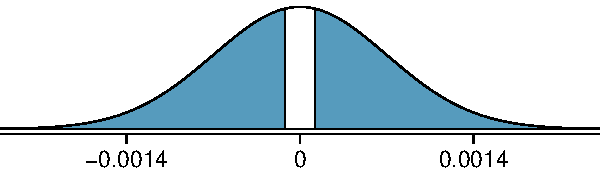
\includegraphics[width=0.6\textwidth]{ch_inference_for_props/figures/mammograms/mammogramPValue}
\end{center}
The lower tail area is 0.4325, which we double to get the p-value:~0.8650. Because this p-value is larger than 0.05, we do not reject the null hypothesis. That is, the difference in breast cancer death rates is reasonably explained by chance, and we do not observe benefits of or harm from mammograms relative to a regular breast exam.
\end{example}

Can we conclude that mammograms have no benefits or harm? Here are a few important considerations to keep in mind when reviewing the mammogram study as well as any other medical study:
\begin{itemize}
\setlength{\itemsep}{0mm}
\item If mammograms are helpful or harmful, the data indicate that the effect isn't very large. So while we do not accept the null hypothesis, it is reasonable to say that mammograms do not reduce or increase breast cancer deaths, if we believe the study participants are reasonably representative of the population. We could also compute a confidence interval to give a sense of the plausible impact of mammograms.
\item Are mammograms more or less expensive than a non-mammogram breast exam? If one option is much more expensive than the other and doesn't offer clear benefits, then we should lean towards the less expensive option.
\item The study also found that mammograms led to overdiagnosis of breast cancer, which means some breast cancers were found (or thought to be found) but that these cancers would not cause symptoms during patients' lifetimes. That is, something else would kill the patient before breast cancer symptoms appeared. This means some patients may have been treated for breast cancer unnecessarily, and this treatment is another cost to consider. It is also important to recognize that overdiagnosis can cause unnecessary physical or emotional harm to patients.
\end{itemize}
These considerations highlight the complexity around medical care and treatment recommendations. Experts and medical boards who study medical treatments use considerations like those above to provide their best recommendation based on the current evidence.

%\begin{caution}{Practical consideration on scientific research}
%{Recognize that there may be deeper complexities to a problem than a simple hypothesis test. This is especially true in medical research. For example, even if one treatment is very effective, if it is far too costly, it may not be a viable treatmen}
%\end{caution}

%The second consideration mentioned in Example~\ref{} -- the cost of a test and cost of overdiagnosis -- are frequently important in medical care, even.

\index{data!breast cancer|)}
\index{data!mammography|)}

\CalculatorVideos{confidence intervals and hypothesis tests for the difference of two proportion}


\subsection{More on 2-proportion hypothesis tests (special topic)}

When we conduct a 2-proportion hypothesis test, usually $H_0$ is $p_1 - p_2 = 0$. However, there are rare situations where we want to check for some difference in $p_1$ and $p_2$ that is some value other than 0. For example, maybe we care about checking a null hypothesis where $p_1 - p_2 = 0.1$.\footnote{We can also encounter a similar situation with a difference of two means, though no such example was given in Chapter~\ref{inferenceForNumericalData} since the methods remain exactly the same in that context whereas the success-failure condition and the calculation of the standard error vary slightly in different proportion contexts.} In contexts like these, we generally use $\hat{p}_1$ and $\hat{p}_2$ to check the success-failure condition and construct the standard error.

\begin{exercise}\label{carWheelBladeManufacturer}
A quadcopter company is considering a new manufacturer for rotor blades. The new manufacturer would be more expensive but their higher-quality blades are more reliable, resulting in happier customers and fewer warranty claims. However, management must be convinced that the more expensive blades are worth the conversion before they approve the switch. If there is strong evidence of a more than 3\% improvement in the percent of blades that pass inspection, management says they will switch suppliers, otherwise they will maintain the current supplier. Set up appropriate hypotheses for the test.\footnote{$H_0$: The higher-quality blades will pass inspection no more than 3\% more frequently than the standard-quality blades. $p_{highQ} - p_{standard} = 0.03$. $H_A$: The higher-quality blades will pass inspection more than 3\% more often than the standard-quality blades. $p_{highQ} - p_{standard} > 0.03$.}
\end{exercise}

\setlength{\captionwidth}{85mm}

\begin{figure}
\centering
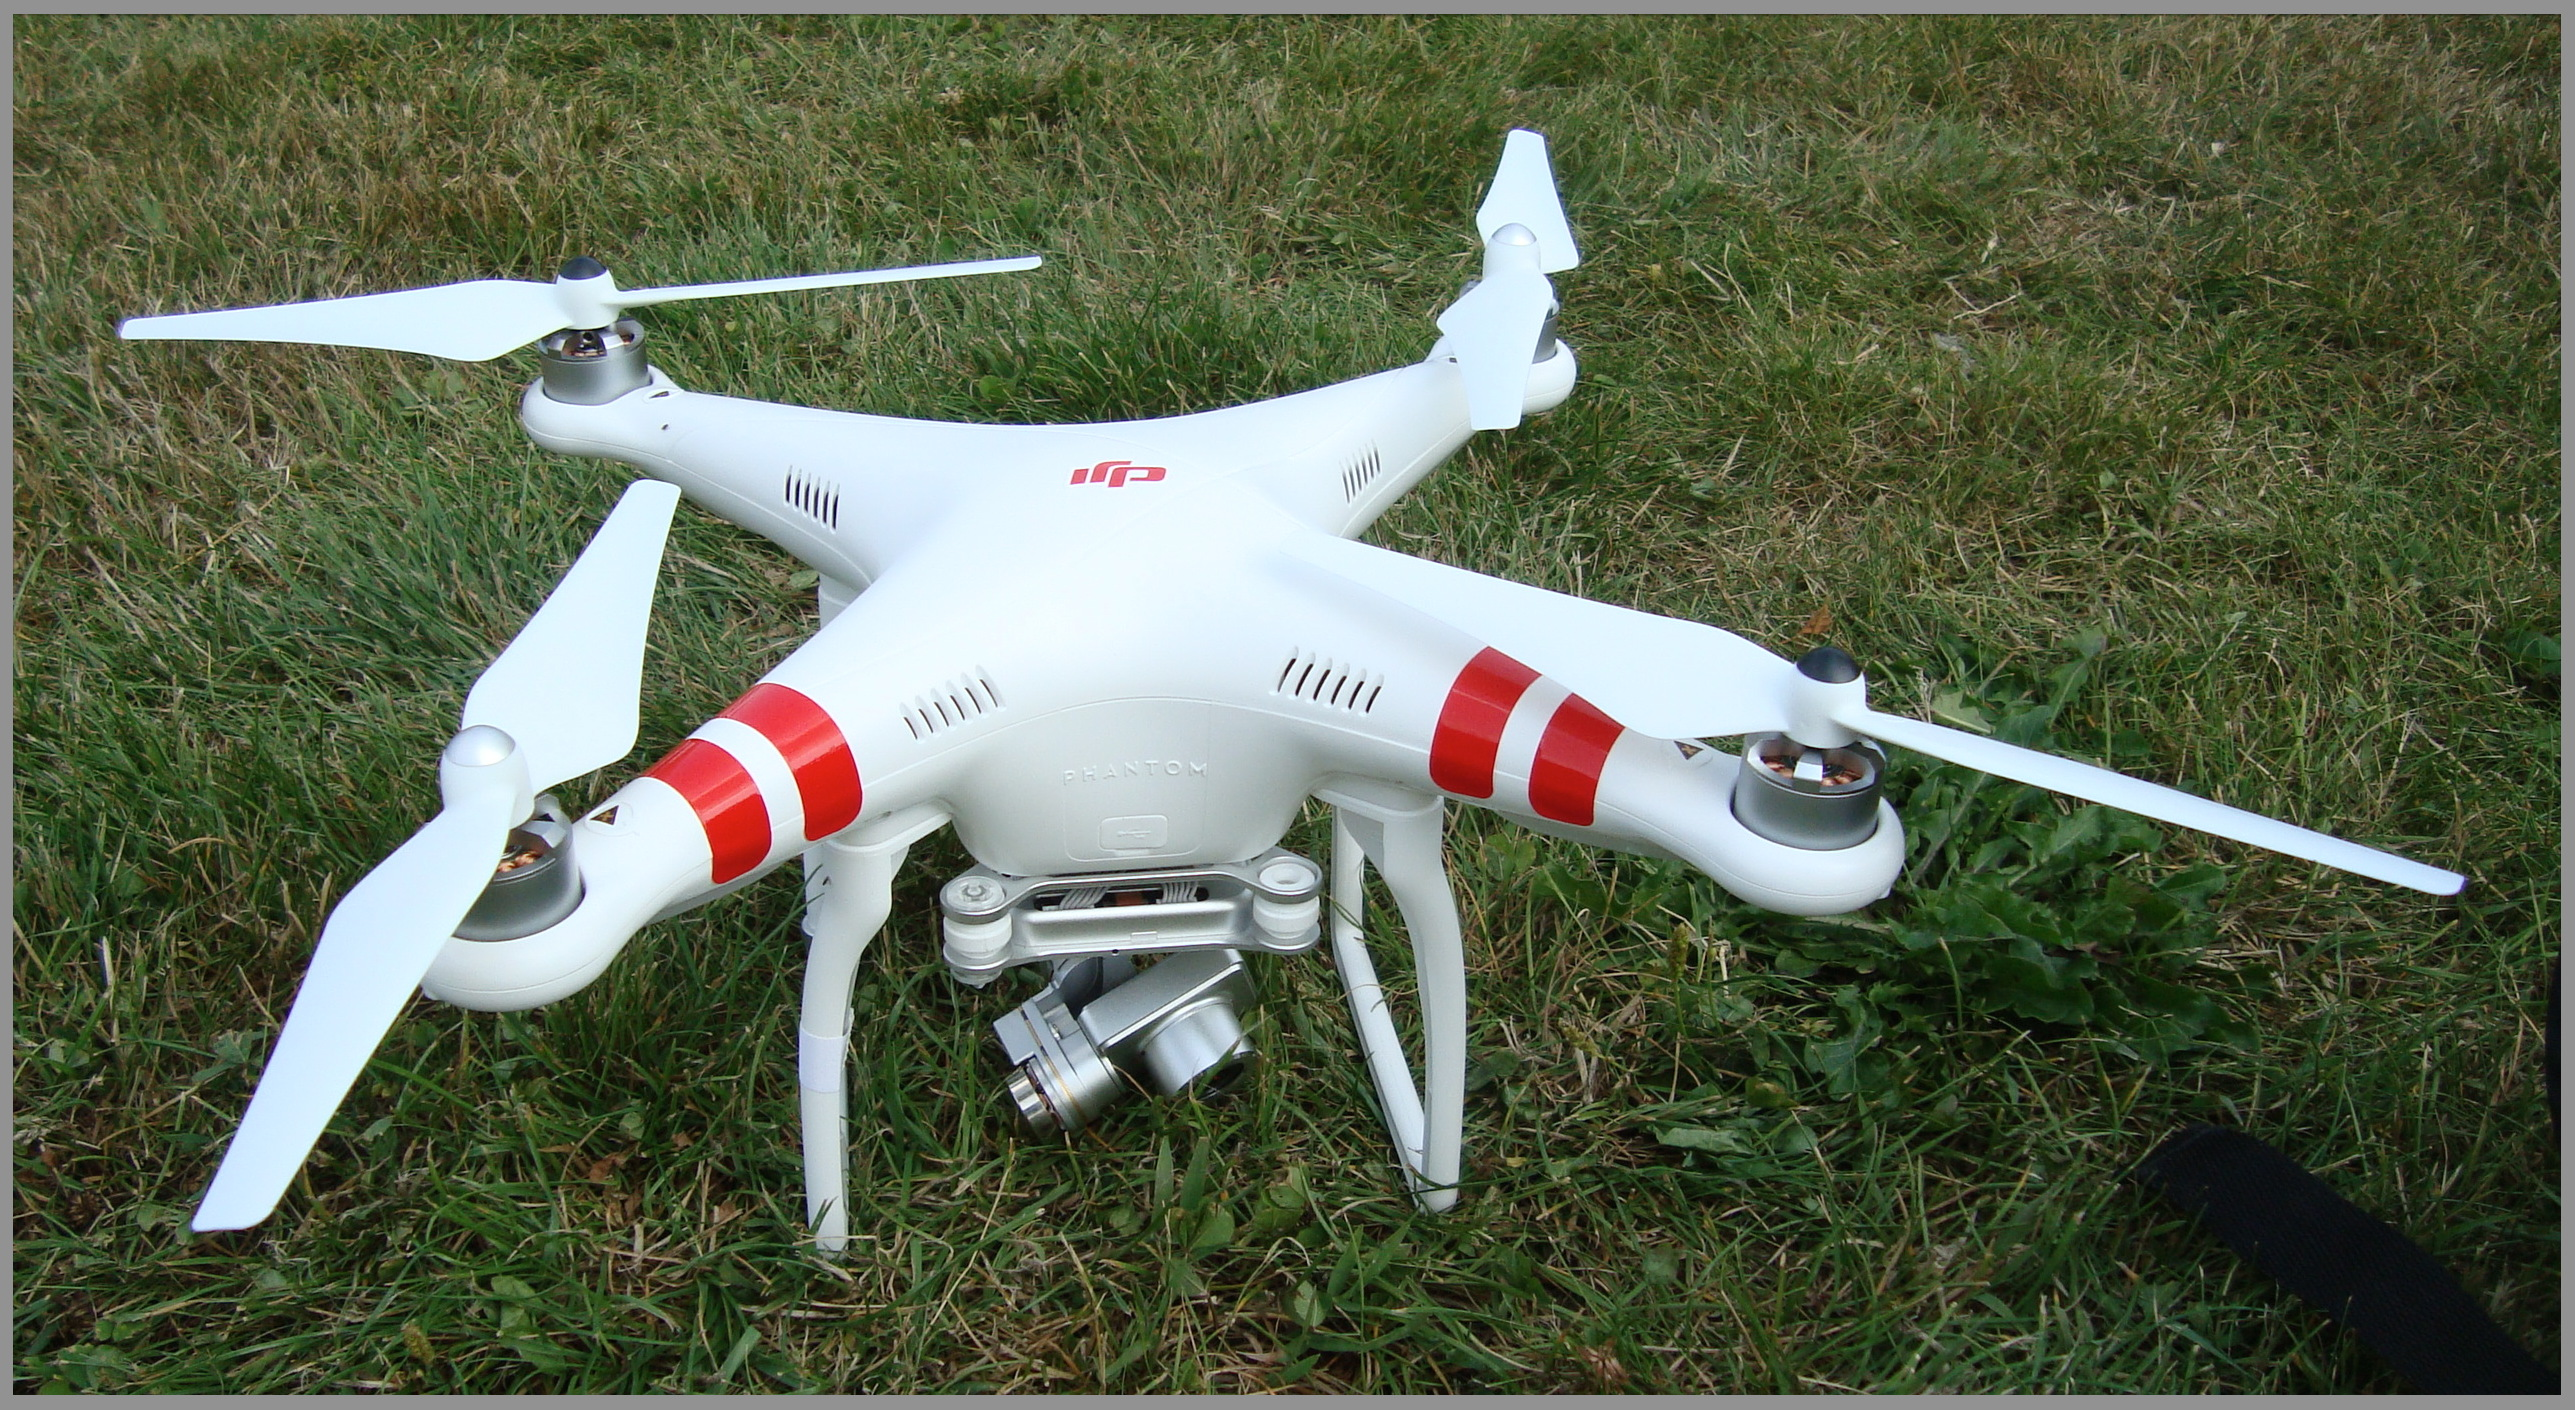
\includegraphics[width=0.6\textwidth]{ch_inference_for_props/figures/quadcopter/quadcopter_david_j}
\caption{A Phantom quadcopter.\vspace{-1mm} \\
   -----------------------------\vspace{-2mm}\\
   {\footnotesize Photo by David J (\oiRedirect{textbook-quadcopter_david_j}{http://flic.kr/p/oiWLNu}). \oiRedirect{textbook-CC_BY_2}{CC-BY 2.0 license.} This photo has been cropped and a border has been added.}}
\label{quadcopter_david_j}
\end{figure}

\setlength{\captionwidth}{\mycaptionwidth}

%\Add{In Guided Practice~\ref{qualityCtrlEngHypothesisEval}, the null difference is 0.03. However, in the vast majority of applications for differences in means or proportions, the null difference is~0. While the details for a difference of means does not change if the null difference is zero or non-zero, that is not the case for a difference in proportions. As we'll see in Section~\ref{}, a hypothesis test for a difference in proportions where the null value is 0 requires additional~care.}

\begin{example}{The quality control engineer from Guided Practice~\ref{carWheelBladeManufacturer} collects a sample of blades, examining 1000 blades from each company and finds that 899 blades pass inspection from the current supplier and 958 pass inspection from the prospective supplier. Using these data, evaluate the hypothesis setup of Guided Practice~\ref{carWheelBladeManufacturer} using a significance level of 5\%.}\label{qualityCtrlEngHypothesisEval}
First, we check the conditions. The sample is not necessarily random, so to proceed we must assume the blades are all independent; for this sample we will suppose this assumption is reasonable, but the engineer would be more knowledgeable as to whether this assumption is appropriate. The success-failure condition also holds for each sample. Thus, the difference in sample proportions, $0.958 - 0.899 = 0.059$, can be said to come from a nearly normal distribution.

The standard error can be found using Equation~\eqref{seForDiffOfProp}:
\begin{align*}
SE = \sqrt{\frac{0.958(1-0.958)}{1000} + \frac{0.899(1-0.899)}{1000}} = 0.0114
\end{align*}
In this hypothesis test, because the null is that $p_1 - p_2 = 0.03$, the sample proportions were used for the standard error calculation rather than a pooled proportion.

Next, we compute the test statistic and use it to find the p-value, which is depicted in Figure~\ref{bladesTwoSampleHTPValueQC}.
$$Z = \frac{\text{point estimate} - \text{null value}}{SE} = \frac{0.059 - 0.03}{0.0114} = 2.54$$
Using the normal model for this test statistic, we identify the right tail area as 0.006. Since this is a one-sided test, this single tail area is also the p-value, and we reject the null hypothesis because 0.006 is less than 0.05. That is, we have statistically significant evidence that the higher-quality blades actually do pass inspection more than 3\% as often as the currently used blades. Based on these results, management will approve the switch to the new supplier.
\end{example}

\begin{figure}
\centering
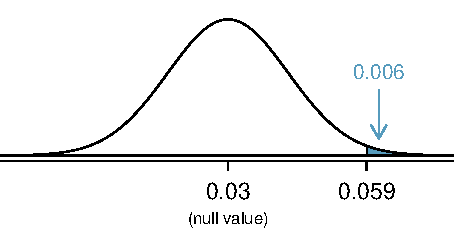
\includegraphics[width=0.5\textwidth]{ch_inference_for_props/figures/bladesTwoSampleHTPValueQC/bladesTwoSampleHTPValueQC}
\caption{Distribution of the test statistic if the null hypothesis was true. The p-value is represented by the shaded area.}
\label{bladesTwoSampleHTPValueQC}
\end{figure}



%%__________________
%\section{Determining a sample size for an experiment}
%\label{SampleSizeFor2Proportions}
%
%So far we've been focused on controlling the Type~1 Error rate for hypothesis tests. However, when planning an experiment, we often are interested in determining if there is an effect.\footnote{Similar planning is also appropriate for a} There are often two competing considerations:
%\begin{itemize}
%\setlength{\itemsep}{0mm}
%\item We want to collect enough data that we can detect important effects.
%\item In many contexts, collecting data is expensive, so we don't want to collect more than what we need to detect effects we care about.
%\end{itemize}
%The first point is relatively simple: the more data we collect, the more precise our estimates will be, and so we'll be able to detect smaller effects. The second point is more subtle, since we need to determine the size of effects that we care about.
%
%%\begin{example}{Alzheimer's disease is a neurological disease. It affects patients mildly at the beginning and eventually leads to dementia. If an Alzheimer's patient lives long enough, the disease will begin affecting bodily functions and ultimately lead to death. It's an extremely serious condition that millions of people, has no cure, and is very expensive to research, partially due to its slow progression. A group of researchers is }
%\begin{example}{}
%
%\end{example}
%
%
%, even large ones, are difficult to detect with small samples, so we should want to collect a larger sample to detect such effects. If we take a very large sample, we might find a statistically significant difference but the magnitude might be so small that it is of no practical value. In this section we describe techniques for selecting an appropriate sample size based on these considerations.



%__________________
\section[Testing for goodness of fit using chi-square (special topic)]{Testing for goodness of fit using chi-square \\(special topic)}
\label{oneWayChiSquare}

In this section, we develop a method for assessing a null model when the data are binned.
This technique is commonly used in two circumstances:
\begin{itemize}
\setlength{\itemsep}{0mm}
\item Given a sample of cases that can be classified into several groups, determine if the sample is representative of the general population.
\item Evaluate whether data resemble a particular distribution, such as a normal distribution or a geometric distribution.
\end{itemize}
Each of these scenarios can be addressed using the same statistical test: a chi-square test.

\index{data!racial make-up of jury|(}

In the first case, we consider data from a random sample of 275 jurors in a small county. Jurors identified their racial group, as shown in Table~\ref{juryRepresentationAndCityRepresentationForRace}, and we would like to determine if these jurors are racially representative of the population.  If the jury is representative of the population, then the proportions in the sample should roughly reflect the population of eligible jurors, i.e. registered voters.

\begin{table}[h]
\centering
\begin{tabular}{ll ccc c ll}
\hline
Race	 & \hspace{2mm} & White & Black & Hispanic & Other & \hspace{2mm} & Total \\
\hline
Representation in juries &	& 205 & 26 & 25 & 19 & & 275 \\
Registered voters	 & 		& 0.72 & 0.07 & 0.12 & 0.09 & & 1.00 \\
\hline
\end{tabular}
\caption{Representation by race in a city's juries and population.}
\label{juryRepresentationAndCityRepresentationForRace}
\end{table}

While the proportions in the juries do not precisely represent the population proportions, it is unclear whether these data provide convincing evidence that the sample is not representative. If the jurors really were randomly sampled from the registered voters, we might expect small differences due to chance. However, unusually large differences may provide convincing evidence that the juries were not representative.

A second application, assessing the fit of a distribution, is presented at the end of this section. Daily stock returns from the S\&P500 for the years 1990-2011 are used to assess whether stock activity each day is independent of the stock's behavior on previous days.

In these problems, we would like to examine all bins simultaneously, not simply compare one or two bins at a time, which will require us to develop a new test statistic.


\subsection{Creating a test statistic for one-way tables}

\begin{example}{Of the people in the city, 275 served on a jury. If the individuals are randomly selected to serve on a jury, about how many of the 275 people would we expect to be white? How many would we expect to be black?}
About 72\% of the population is white, so we would expect about 72\% of the jurors to be white: $0.72\times 275 = 198$.

Similarly, we would expect about 7\% of the jurors to be black, which would correspond to about $0.07\times 275 = 19.25$ black jurors.
\end{example}

\begin{exercise}
Twelve percent of the population is Hispanic and 9\% represent other races. How many of the 275 jurors would we expect to be Hispanic or from another race? Answers can be found in Table~\ref{expectedJuryRepresentationIfNoBias}.
\end{exercise}

\begin{table}[h]
\centering
\begin{tabular}{ll ccc c ll}
\hline
Race	 & \hspace{2mm} & White & Black & Hispanic & Other & \hspace{2mm} & Total \\
\hline
Observed data			&	& 205 & 26	& 25 & 19	&	& 275 \\
Expected counts	 &	& 198 & 19.25 & 33 & 24.75 & & 275 \\
\hline
\end{tabular}
\caption{Actual and expected make-up of the jurors.}
\label{expectedJuryRepresentationIfNoBias}
\end{table}

The sample proportion represented from each race among the 275 jurors was not a precise match for any ethnic group. While some sampling variation is expected, we would expect the sample proportions to be fairly similar to the population proportions if there is no bias on juries. We need to test whether the differences are strong enough to provide convincing evidence that the jurors are not a random sample. These ideas can be organized into hypotheses:
\begin{itemize}
\setlength{\itemsep}{0mm}
\item[$H_0$:] The jurors are a random sample, i.e. there is no racial bias in who serves on a jury, and the observed counts reflect natural sampling fluctuation.
\item[$H_A$:] The jurors are not randomly sampled, i.e. there is racial bias in juror selection.
\end{itemize}
To evaluate these hypotheses, we quantify how different the observed counts are from the expected counts. Strong evidence for the alternative hypothesis would come in the form of unusually large deviations in the groups from what would be expected based on sampling variation alone.


\subsection{The chi-square test statistic}
\label{chiSquareTestStatistic}

In previous hypothesis tests, we constructed a test statistic of the following form:
$$ \frac{\text{point estimate} - \text{null value}}{\text{SE of point estimate}} $$
This construction was based on (1) identifying the difference between a point estimate and an expected value if the null hypothesis was true, and (2) standardizing that difference using the standard error of the point estimate. These two ideas will help in the construction of an appropriate test statistic for count data.

Our strategy will be to first compute the difference between the observed counts and the counts we would expect if the null hypothesis was true, then we will standardize the difference:
\begin{align*}
Z_{1} = \frac{\text{observed white count} - \text{null white count}}
				{\text{SE of observed white count}}
\end{align*}
The standard error for the point estimate of the count in binned data is the square root of the count under the null.\footnote{Using some of the rules learned in earlier chapters, we might think that the standard error would be $np(1-p)$, where $n$ is the sample size and $p$ is the proportion in the population. This would be correct if we were looking only at one count. However, we are computing many standardized differences and adding them together. It can be shown -- though not here -- that the square root of the count is a better way to standardize the count differences.} Therefore:
\begin{align*}
Z_1 = \frac{205 - 198}{\sqrt{198}} = 0.50
\end{align*}
The fraction is very similar to previous test statistics: first compute a difference, then standardize it. These computations should also be completed for the black, Hispanic, and other groups:
\begin{align*}
&Black && Hispanic	&&Other \\
& Z_2 = \frac{26-19.25}{\sqrt{19.25}}=1.54\ \ \ \ 
	&& Z_3 = \frac{25-33}{\sqrt{33}}=-1.39\ \ \ \ 
	&& Z_4 = \frac{19-24.75}{\sqrt{24.75}}=-1.16 \\
\end{align*}
We would like to use a single test statistic to determine if these four standardized differences are irregularly far from zero. That is, $Z_1$, $Z_2$, $Z_3$, and $Z_4$ must be combined somehow to help determine if they -- as a group -- tend to be unusually far from zero. A first thought might be to take the absolute value of these four standardized differences and add them~up:
\begin{align*}
|Z_1| + |Z_2| + |Z_3| + |Z_4| = 4.58
\end{align*}
Indeed, this does give one number summarizing how far the actual counts are from what was expected. However, it is more common to add the squared values:
\begin{align*}
Z_1^2 + Z_2^2 + Z_3^2 + Z_4^2 = 5.89
\end{align*}
Squaring each standardized difference before adding them together does two things:
\begin{itemize}
\setlength{\itemsep}{0mm}
\item Any standardized difference that is squared will now be positive.
\item Differences that already look unusual -- e.g. a standardized difference of 2.5 -- will become much larger after being squared.
\end{itemize}
The test statistic $\chi^2$\marginpar[\raggedright\vspace{9mm}

$\chi^2$\vspace{0.5mm}\\\footnotesize chi-square\\test statistic]{\raggedright\vspace{9mm}

$\chi^2$\vspace{0.5mm}\\\footnotesize chi-square\\test statistic},\index{chi-square statistic} which is the sum of the $Z^2$ values, is generally used for these reasons. We can also write an equation for $\chi^2$ using the observed counts and null counts:
\index{data!racial make-up of jury|)}
{\begin{align*}
\chi^2 &=
	\frac
	{\text{\footnotesize$(\text{observed count}_1 - \text{null count}_1)^2$}}
	{\text{\footnotesize$\text{null count}_1$}}
	+ \dots + \frac
	{\text{\footnotesize$(\text{observed count}_4 - \text{null count}_4)^2$}}
	{\text{\footnotesize$\text{null count}_4$}}
\end{align*}
}The final number $\chi^2$ summarizes how strongly the observed counts tend to deviate from the null counts. In Section~\ref{pValueForAChiSquareTest}, we will see that if the null hypothesis is true, then $\chi^2$ follows a new distribution called a \emph{chi-square distribution}. Using this distribution, we will be able to obtain a p-value to evaluate the hypotheses.


\subsection{The chi-square distribution and finding areas}

The \term{chi-square distribution} is sometimes used to characterize data sets and statistics that are always positive and typically right skewed. Recall the normal distribution had two parameters -- mean and standard deviation -- that could be used to describe its exact characteristics. The chi-square distribution has just one parameter called \termsub{degrees of freedom (df)}{degrees of freedom (df)!chi-square}, which influences the shape, center, and spread of the distribution.

\begin{exercise}\label{exerChiSquareDistributionDescriptionWithMoreDOF}
Figure~\ref{chiSquareDistributionWithInceasingDF} shows three chi-square distributions. (a) How does the center of the distribution change when the degrees of freedom is larger? (b) What about the variability (spread)? (c) How does the shape change?\footnote{(a)~The center becomes larger. If we look carefully, we can see that the center of each distribution is equal to the distribution's degrees of freedom. (b)~The variability increases as the degrees of freedom increases. (c)~The distribution is very strongly skewed for $df=2$, and then the distributions become more symmetric for the larger degrees of freedom $df=4$ and $df=9$. We would see this trend continue if we examined distributions with even more larger degrees of freedom.}
\end{exercise}

\begin{figure}[h]
\centering
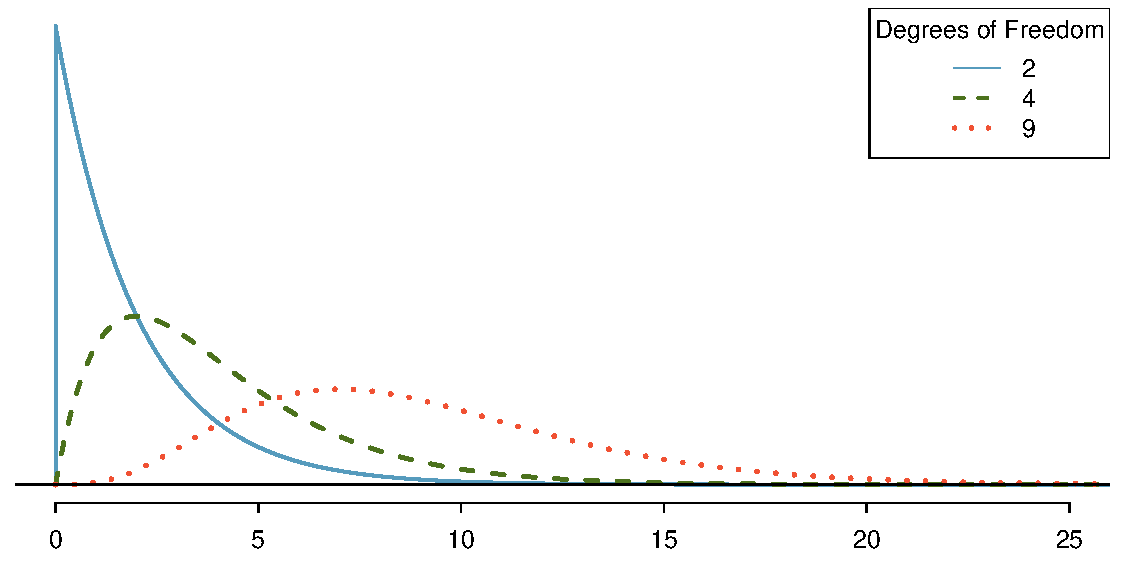
\includegraphics[width=0.9\textwidth]{ch_inference_for_props/figures/chiSquareDistributionWithInceasingDF/chiSquareDistributionWithInceasingDF}
\caption{Three chi-square distributions with varying degrees of freedom.}
\label{chiSquareDistributionWithInceasingDF}
\end{figure}

Figure~\ref{chiSquareDistributionWithInceasingDF} and Guided Practice~\ref{exerChiSquareDistributionDescriptionWithMoreDOF} demonstrate three general properties of chi-square distributions as the degrees of freedom increases: the distribution becomes more symmetric, the center moves to the right, and the variability inflates.

Our principal interest in the chi-square distribution is the calculation of p-values, which (as we have seen before) is related to finding the relevant area in the tail of a distribution. To do so, a new table is needed: the \term{chi-square table}, partially shown in Table~\ref{chiSquareProbabilityTableShort}. A more complete table is presented in Appendix~\vref{chiSquareProbabilityTable}. This table is very similar to the $t$ table from Sections~\ref{oneSampleMeansWithTDistribution} and~\ref{theTDistributionForTheDifferenceOfTwoMeans}: we identify a range for the area, and we examine a particular row for distributions with different degrees of freedom. One important difference from the $t$ table is that the chi-square table only provides upper tail values.

\begin{table}[h]
\centering
\begin{tabular}{r | rrrr | rrrr |}
  \hline
Upper tail & 0.3 & 0.2 & 0.1 & 0.05 & 0.02 & 0.01 & 0.005 & 0.001 \\ 
  \hline
%df \hfill 1 & \footnotesize 1.07 & \footnotesize 1.64 & \footnotesize 2.71 & \footnotesize 3.84 & \footnotesize 5.41 & \footnotesize 6.63 & \footnotesize 7.88 & \footnotesize 10.83 \\ 
df \hfill 2 & \footnotesize 2.41 & \footnotesize \highlightO{3.22} & \footnotesize \highlightO{4.61} & \footnotesize 5.99 & \footnotesize 7.82 & \footnotesize 9.21 & \footnotesize 10.60 & \footnotesize 13.82 \\ 
  \em3 & \em\footnotesize 3.66 & \em\footnotesize 4.64 & \em\footnotesize \highlightT{6.25} & \em\footnotesize 7.81 & \em\footnotesize 9.84 & \em\footnotesize 11.34 & \em\footnotesize 12.84 & \em\footnotesize 16.27 \\ 
  4 & \footnotesize 4.88 & \footnotesize 5.99 & \footnotesize 7.78 & \footnotesize 9.49 & \footnotesize 11.67 & \footnotesize 13.28 & \footnotesize 14.86 & \footnotesize 18.47 \\ 
  5 & \footnotesize 6.06 & \footnotesize 7.29 & \footnotesize 9.24 & \footnotesize 11.07 & \footnotesize 13.39 & \footnotesize 15.09 & \footnotesize 16.75 & \footnotesize 20.52 \\ 
  \hline
  6 & \footnotesize 7.23 & \footnotesize 8.56 & \footnotesize 10.64 & \footnotesize 12.59 & \footnotesize 15.03 & \footnotesize 16.81 & \footnotesize 18.55 & \footnotesize 22.46 \\ 
  7 & \footnotesize 8.38 & \footnotesize 9.80 & \footnotesize 12.02 & \footnotesize 14.07 & \footnotesize 16.62 & \footnotesize 18.48 & \footnotesize 20.28 & \footnotesize 24.32 \\ 
  \hline
\end{tabular}
\caption{A section of the chi-square table. A complete table is in Appendix~\vref{chiSquareProbabilityTable}.}
\label{chiSquareProbabilityTableShort}
\end{table}

\begin{example}{Figure~\ref{chiSquareAreaAbove6Point25WithDF3} shows a chi-square distribution with 3 degrees of freedom and an upper shaded tail starting at 6.25. Use Table~\ref{chiSquareProbabilityTableShort} to estimate the shaded area.}
This distribution has three degrees of freedom, so only the row with 3 degrees of freedom (df) is relevant. This row has been italicized in the table. Next, we see that the value -- 6.25 -- falls in the column with upper tail area 0.1. That is, the shaded upper tail of Figure~\ref{chiSquareAreaAbove6Point25WithDF3} has area 0.1.
\end{example}

\begin{figure}
\centering
\subfigure[]{
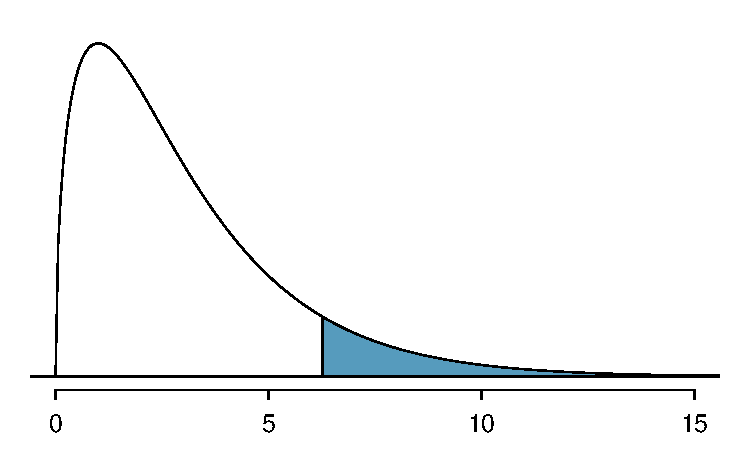
\includegraphics[width=0.475\textwidth]{ch_inference_for_props/figures/arrayOfFigureAreasForChiSquareDistribution/chiSquareAreaAbove6Point25WithDF3/chiSquareAreaAbove6Point25WithDF3}
\label{chiSquareAreaAbove6Point25WithDF3}
}
\subfigure[]{
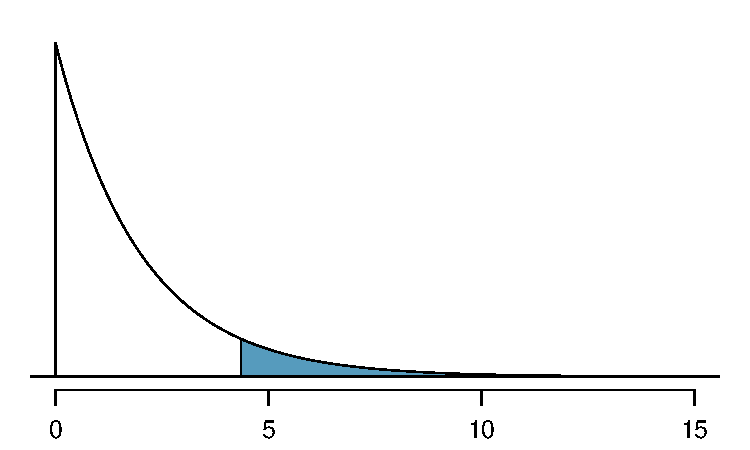
\includegraphics[width=0.475\textwidth]{ch_inference_for_props/figures/arrayOfFigureAreasForChiSquareDistribution/chiSquareAreaAbove4Point3WithDF2/chiSquareAreaAbove4Point3WithDF2}
\label{chiSquareAreaAbove4Point3WithDF2}
}
\subfigure[]{
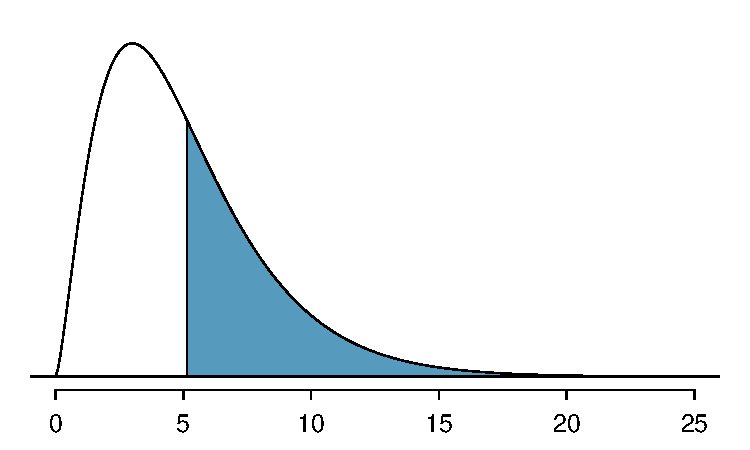
\includegraphics[width=0.475\textwidth]{ch_inference_for_props/figures/arrayOfFigureAreasForChiSquareDistribution/chiSquareAreaAbove5Point1WithDF5/chiSquareAreaAbove5Point1WithDF5}
\label{chiSquareAreaAbove5Point1WithDF5}
}
\subfigure[]{
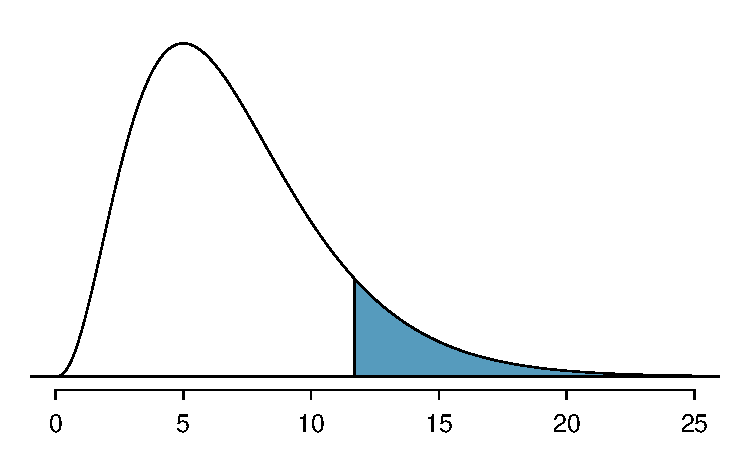
\includegraphics[width=0.475\textwidth]{ch_inference_for_props/figures/arrayOfFigureAreasForChiSquareDistribution/chiSquareAreaAbove11Point7WithDF7/chiSquareAreaAbove11Point7WithDF7}
\label{chiSquareAreaAbove11Point7WithDF7}
}
\subfigure[]{
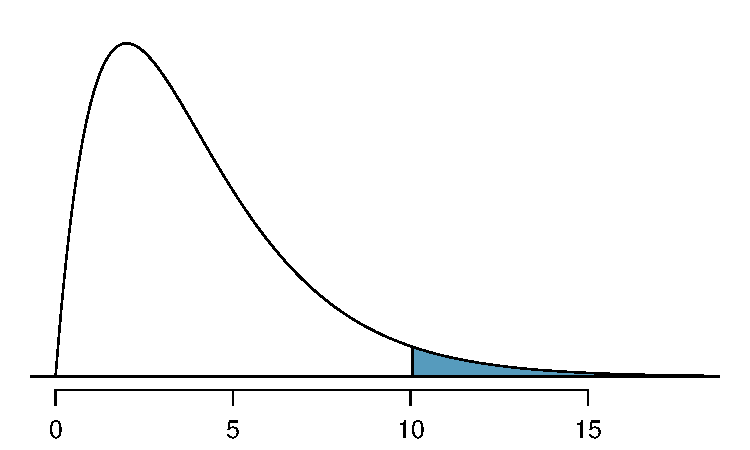
\includegraphics[width=0.475\textwidth]{ch_inference_for_props/figures/arrayOfFigureAreasForChiSquareDistribution/chiSquareAreaAbove10WithDF4/chiSquareAreaAbove10WithDF4}
\label{chiSquareAreaAbove10WithDF4}
}
\subfigure[]{
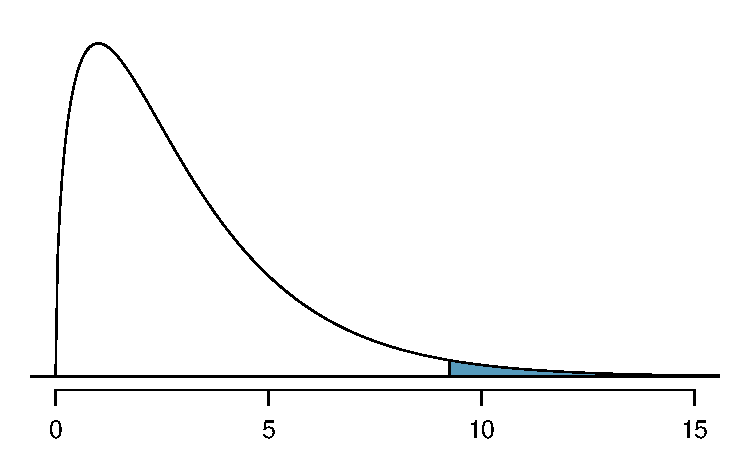
\includegraphics[width=0.475\textwidth]{ch_inference_for_props/figures/arrayOfFigureAreasForChiSquareDistribution/chiSquareAreaAbove9Point21WithDF3/chiSquareAreaAbove9Point21WithDF3}
\label{chiSquareAreaAbove9Point21WithDF3}
}
\caption{\textbf{\subref{chiSquareAreaAbove6Point25WithDF3}} Chi-square distribution with 3 degrees of freedom, area above 6.25 shaded. \textbf{\subref{chiSquareAreaAbove4Point3WithDF2}} 2 degrees of freedom, area above 4.3 shaded. \textbf{\subref{chiSquareAreaAbove5Point1WithDF5}} 5 degrees of freedom, area above 5.1 shaded. \textbf{\subref{chiSquareAreaAbove11Point7WithDF7}} 7 degrees of freedom, area above 11.7 shaded. \textbf{\subref{chiSquareAreaAbove10WithDF4}} 4 degrees of freedom, area above 10 shaded. \textbf{\subref{chiSquareAreaAbove9Point21WithDF3}} 3 degrees of freedom, area above 9.21 shaded.}
\label{arrayOfFigureAreasForChiSquareDistribution}
\end{figure}

\begin{example}{We rarely observe the \emph{exact} value in the table. For instance, Figure~\ref{chiSquareAreaAbove4Point3WithDF2} shows the upper tail of a chi-square distribution with 2 degrees of freedom. The bound for this upper tail is at 4.3, which does not fall in Table~\ref{chiSquareProbabilityTableShort}. Find the approximate tail area.}
The cutoff 4.3 falls between the second and third columns in the 2 degrees of freedom row. Because these columns correspond to tail areas of 0.2 and 0.1, we can be certain that the area shaded in Figure~\ref{chiSquareAreaAbove4Point3WithDF2} is between 0.1 and 0.2.
\end{example}

\begin{example}{Figure~\ref{chiSquareAreaAbove5Point1WithDF5} shows an upper tail for a chi-square distribution with 5 degrees of freedom and a cutoff of 5.1. Find the tail area.}
Looking in the row with 5 df, 5.1 falls below the smallest cutoff for this row (6.06). That means we can only say that the area is \emph{greater than 0.3}.
\end{example}

\begin{exercise}
Figure~\ref{chiSquareAreaAbove11Point7WithDF7} shows a cutoff of 11.7 on a chi-square distribution with 7 degrees of freedom. Find the area of the upper tail.\footnote{The value 11.7 falls between 9.80 and 12.02 in the 7 df row. Thus, the area is between 0.1 and 0.2.}
\end{exercise}

\begin{exercise}
Figure~\ref{chiSquareAreaAbove10WithDF4} shows a cutoff of 10 on a chi-square distribution with 4 degrees of freedom. Find the area of the upper tail.\footnote{The area is between 0.02 and 0.05.}
\end{exercise}

\begin{exercise}
Figure~\ref{chiSquareAreaAbove9Point21WithDF3} shows a cutoff of 9.21 with a chi-square distribution with 3 df. Find the area of the upper tail.\footnote{Between 0.02 and 0.05.}
\end{exercise}


\subsection{Finding a p-value for a chi-square distribution}
\label{pValueForAChiSquareTest}

\index{data!racial make-up of jury|(}
In Section~\ref{chiSquareTestStatistic}, we identified a new test statistic ($\chi^2$) within the context of assessing whether there was evidence of racial bias in how jurors were sampled. The null hypothesis represented the claim that jurors were randomly sampled and there was no racial bias. The alternative hypothesis was that there was racial bias in how the jurors were sampled.

We determined that a large $\chi^2$ value would suggest strong evidence favoring the alternative hypothesis: that there was racial bias. However, we could not quantify what the chance was of observing such a large test statistic ($\chi^2=5.89$) if the null hypothesis actually was true. This is where the chi-square distribution becomes useful. If the null hypothesis was true and there was no racial bias, then $\chi^2$ would follow a chi-square distribution, with three degrees of freedom in this case. Under certain conditions, the statistic $\chi^2$ follows a chi-square distribution with $k - 1$ degrees of freedom, where $k$ is the number of bins.

\begin{example}{How many categories were there in the juror example? How many degrees of freedom should be associated with the chi-square distribution used for $\chi^2$?}
In the jurors example, there were $k=4$ categories: white, black, Hispanic, and other. According to the rule above, the test statistic $\chi^2$ should then follow a chi-square distribution with $k-1 = 3$ degrees of freedom if $H_0$ is true.
\end{example}

Just like we checked sample size conditions to use the normal model in earlier sections, we must also check a sample size condition to safely apply the chi-square distribution for $\chi^2$. Each expected count must be at least 5. In the juror example, the expected counts were 198, 19.25, 33, and 24.75, all easily above~5, so we can apply the chi-square model to the test statistic, $\chi^2=5.89$.

\begin{example}{If the null hypothesis is true, the test statistic $\chi^2=5.89$ would be closely associated with a chi-square distribution with three degrees of freedom. Using this distribution and test statistic, identify the p-value.}
The chi-square distribution and p-value are shown in Figure~\ref{jurorHTPValueShown}. Because larger chi-square values correspond to stronger evidence against the null hypothesis, we shade the upper tail to represent the p-value. Using the chi-square table in Appendix~\ref{chiSquareProbabilityTable} or the short table on page~\pageref{chiSquareProbabilityTableShort}, we can determine that the area is between 0.1 and 0.2. That is, the p-value is larger than 0.1 but smaller than 0.2. Generally we do not reject the null hypothesis with such a large p-value. In other words, the data do not provide convincing evidence of racial bias in the juror selection.
\index{data!racial make-up of jury|)}
\end{example}

\begin{figure}[h]
\centering
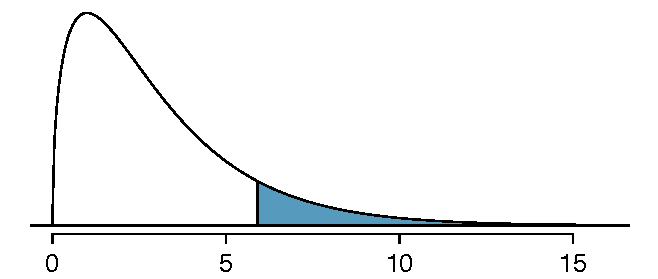
\includegraphics[width=0.61\textwidth]{ch_inference_for_props/figures/jurorHTPValueShown/jurorHTPValueShown}
\caption{The p-value for the juror hypothesis test is shaded in the chi-square distribution with $df=3$.}
\label{jurorHTPValueShown}
\end{figure}

\begin{termBox}{\tBoxTitle{Chi-square test for one-way table}
Suppose we are to evaluate whether there is convincing evidence that a set of observed counts $O_1$, $O_2$, ..., $O_k$ in $k$ categories are unusually different from what might be expected under a null hypothesis. Call the \emph{expected counts} that are based on the null hypothesis $E_1$, $E_2$, ..., $E_k$. If each expected count is at least 5 and the null hypothesis is true, then the test statistic below follows a chi-square distribution with $k-1$ degrees of freedom:
\begin{align*}
\chi^2 = \frac{(O_1 - E_1)^2}{E_1} + \frac{(O_2 - E_2)^2}{E_2} + \cdots + \frac{(O_k - E_k)^2}{E_k}
\end{align*}
The p-value for this test statistic is found by looking at the upper tail of this chi-square distribution. We consider the upper tail because larger values of $\chi^2$ would provide greater evidence against the null hypothesis.}
\end{termBox}

\begin{tipBox}{\tipBoxTitle{Conditions for the chi-square test}
There are two conditions that must be checked before performing a chi-square test:\vspace{-1mm}
\begin{description}
\setlength{\itemsep}{0mm}
\item[Independence.] Each case that contributes a count to the table must be independent of all the other cases in the table.
\item[Sample size / distribution.] Each particular scenario (i.e. cell count) must have at least 5~expected cases.
\vspace{-1mm}
\end{description}
Failing to check conditions may affect the test's error rates.}
\end{tipBox}

When examining a table with just two bins, pick a single bin and use the one-proportion methods introduced in Section~\ref{singleProportion}.


\subsection{Evaluating goodness of fit for a distribution}

Section~\ref{geomDist} would be useful background reading for this example, but it is not a prerequisite.

\index{data!S\&P500 stock data|(}

We can apply our new chi-square testing framework to the second problem in this section: evaluating whether a certain statistical model fits a data set. Daily stock returns from the S\&P500 for 1990-2011 can be used to assess whether stock activity each day is independent of the stock's behavior on previous days. This sounds like a very complex question, and it is, but a chi-square test can be used to study the problem. We will label each day as \resp{Up} or \resp{Down} (\resp{D}) depending on whether the market was up or down that day. For example, consider the following changes in price, their new labels of up and down, and then the number of days that must be observed before each \resp{Up} day:
\begin{center}\footnotesize
\begin{tabular}{lc ccc ccc ccc cc}
Change in price		&\hspace{-1mm}	& \footnotesize2.52 &
	\footnotesize-1.46 & \footnotesize 0.51 &
	\footnotesize-4.07 & \footnotesize3.36 &
	\footnotesize1.10 &
	\footnotesize-5.46 & \footnotesize-1.03 & \footnotesize-2.99 & \footnotesize1.71 \\
Outcome	 & \hspace{-1mm} &
	Up &
	D & Up &
	D & Up &
	Up &
	D & D & D & Up \\
\footnotesize Days to Up & \hspace{-1mm} & 1 & - & 2 & - & 2 & 1 & - & - & - & 4 \\
\end{tabular}
\end{center}
If the days really are independent, then the number of days until a positive trading day should follow a geometric distribution. The geometric distribution describes the probability of waiting for the $k^{th}$ trial to observe the first success. Here each up day (Up) represents a success, and down (D) days represent failures. In the data above, it took only one day until the market was up, so the first wait time was 1 day. It took two more days before we observed our next \resp{Up} trading day, and two more for the third \resp{Up} day. We would like to determine if these counts (1, 2, 2, 1, 4, and so on) follow the geometric distribution. Table~\ref{sAndP500For1990To2011TimeToPosTrade} shows the number of waiting days for a positive trading day during 1990-2011 for the S\&P500.

\begin{table}[h]
\centering
\begin{tabular}{ll ccc ccc c ll}
\hline
Days	 & \hspace{2mm} & 1 & 2 & 3 & 4 & 5 & 6 & 7+ & \hspace{2mm} & Total \\
Observed &		& 1532 & 760 & 338 & 194 & 74 & 33 & 17 & & 2948 \\
\hline
\end{tabular}
\caption{Observed distribution of the waiting time until a positive trading day for the S\&P500, 1990-2011.}
\label{sAndP500For1990To2011TimeToPosTrade}
\end{table}

We consider how many days one must wait until observing an \resp{Up} day on the S\&P500 stock index. If the stock activity was independent from one day to the next and the probability of a positive trading day was constant, then we would expect this waiting time to follow a \emph{geometric distribution}. We can organize this into a hypothesis framework:
\begin{itemize}
\item[$H_0$:] The stock market being up or down on a given day is independent from all other days. We will consider the number of days that pass until an \resp{Up} day is observed. Under this hypothesis, the number of days until an \resp{Up} day should follow a geometric distribution.
\item[$H_A$:] The stock market being up or down on a given day is not independent from all other days. Since we know the number of days until an \resp{Up} day would follow a geometric distribution under the null, we look for deviations from the geometric distribution, which would support the alternative hypothesis.
\end{itemize}
There are important implications in our result for stock traders: if information from past trading days is useful in telling what will happen today, that information may provide an advantage over other traders.

We consider data for the S\&P500 from 1990 to 2011 and summarize the waiting times in Table~\ref{sAndP500For1990To2011TimeToPosTrade2} and Figure~\ref{geomFitEvaluationForSP500For1990To2011}. The S\&P500 was positive on 53.2\% of those days.

\begin{table}
\centering
\begin{tabular}{ll ccc ccc c ll}
\hline
Days	 & \hspace{1mm} & 1 & 2 & 3 & 4 & 5 & 6 & 7+ & \hspace{1mm} & Total \\
\hline
Observed &		& 1532 & 760 & 338 & 194 & 74 & 33 & 17 & & 2948 \\
Geometric Model &		& 1569 & 734 & 343 & 161 & 75 & 35 & 31 & & 2948 \\
\hline
\end{tabular}
\caption{Distribution of the waiting time until a positive trading day. The expected counts based on the geometric model are shown in the last row. To find each expected count, we identify the probability of waiting $D$ days based on the geometric model ($P(D) = (1-0.532)^{D-1}(0.532)$) and multiply by the total number of streaks, 2948. For example, waiting for three days occurs under the geometric model about $0.468^2\times 0.532 = 11.65\%$ of the time, which corresponds to $0.1165\times 2948 = 343$ streaks.}
\label{sAndP500For1990To2011TimeToPosTrade2}
\end{table}

\begin{figure}
\centering
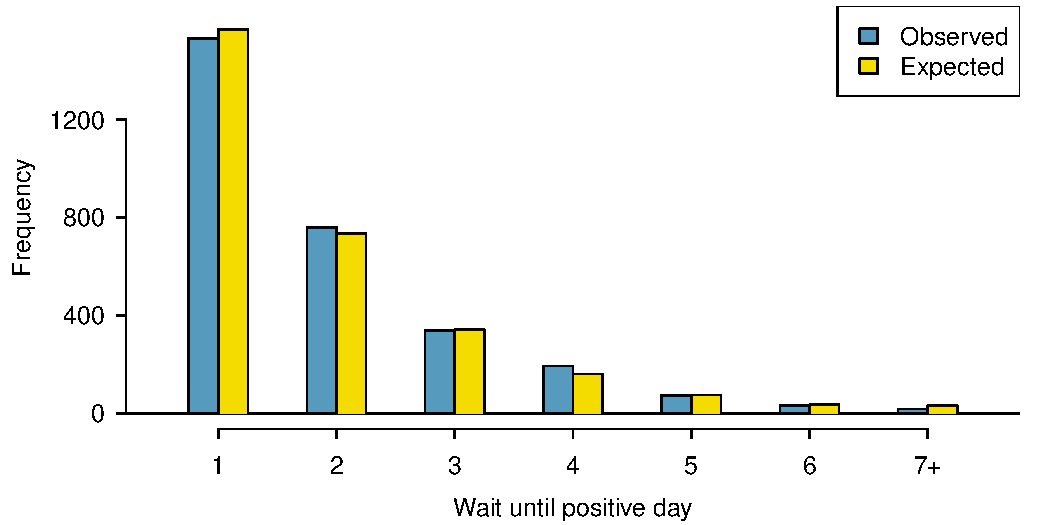
\includegraphics[width=0.98\textwidth]{ch_inference_for_props/figures/geomFitEvaluationForSP500For1990To2011/geomFitEvaluationForSP500For1990To2011}
\caption{Side-by-side bar plot of the observed and expected counts for each waiting time.}
\label{geomFitEvaluationForSP500For1990To2011}
\end{figure}

Because applying the chi-square framework requires expected counts to be at least~5, we have \emph{binned} together all the cases where the waiting time was at least 7 days to ensure each expected count is well above this minimum. The actual data, shown in the \emph{Observed} row in Table~\ref{sAndP500For1990To2011TimeToPosTrade2}, can be compared to the expected counts from the \emph{Geometric Model} row. The method for computing expected counts is discussed in Table~\ref{sAndP500For1990To2011TimeToPosTrade2}. In general, the expected counts are determined by (1) identifying the null proportion associated with each bin, then (2) multiplying each null proportion by the total count to obtain the expected counts. That is, this strategy identifies what proportion of the total count we would expect to be in each bin.

\begin{example}{Do you notice any unusually large deviations in the graph? Can you tell if these deviations are due to chance just by looking?}
It is not obvious whether differences in the observed counts and the expected counts from the geometric distribution are significantly different. That is, it is not clear whether these deviations might be due to chance or whether they are so strong that the data provide convincing evidence against the null hypothesis. However, we can perform a chi-square test using the counts in Table~\ref{sAndP500For1990To2011TimeToPosTrade2}.
\end{example}

\begin{exercise}
Table~\ref{sAndP500For1990To2011TimeToPosTrade2} provides a set of count data for waiting times ($O_1=1532$, $O_2=760$, ...) and expected counts under the geometric distribution ($E_1=1569$, $E_2=734$, ...). Compute the chi-square test statistic, $\chi^2$.\footnote{$\chi^2=\frac{(1532-1569)^2}{1569} + \frac{(760-734)^2}{734} + \cdots + \frac{(17-31)^2}{31} = 15.08$}
\end{exercise}

\begin{exercise}
Because the expected counts are all at least~5, we can safely apply the chi-square distribution to $\chi^2$. However, how many degrees of freedom should we~use?\footnote{There are $k=7$ groups, so we use $df=k-1=6$.}
\end{exercise}

\begin{example}{If the observed counts follow the geometric model, then the chi-square test statistic $\chi^2=15.08$ would closely follow a chi-square distribution with $df=6$. Using this information, compute a p-value.} \label{RejectGeomModelForSP500StockDataFor1990To2011}
Figure~\ref{geomFitPValueForSP500For1990To2011} shows the chi-square distribution, cutoff, and the shaded p-value. If we look up the statistic $\chi^2=15.08$ in Appendix~\ref{chiSquareProbabilityTable}, we find that the p-value is between 0.01 and 0.02. In other words, we have sufficient evidence to reject the notion that the wait times follow a geometric distribution, i.e. trading days are not independent and past days may help predict what the stock market will do today.
\end{example}

\begin{figure}
\centering
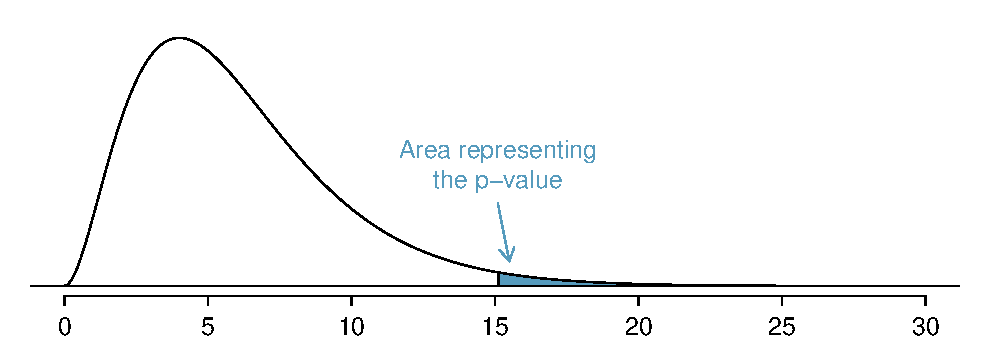
\includegraphics[width=0.97\textwidth]{ch_inference_for_props/figures/geomFitPValueForSP500For1990To2011/geomFitPValueForSP500For1990To2011}
\caption{Chi-square distribution with 6 degrees of freedom. The p-value for the stock analysis is shaded.}
\label{geomFitPValueForSP500For1990To2011}
\end{figure}

\begin{example}{In Example~\ref{RejectGeomModelForSP500StockDataFor1990To2011}, we rejected the null hypothesis that the trading days are independent. Why is this so important?}
Because the data provided strong evidence that the geometric distribution is not appropriate, we reject the claim that trading days are independent. While it is not obvious how to exploit this information, it suggests there are some hidden patterns in the data that could be interesting and possibly useful to a stock trader.
\index{data!S\&P500 stock data|)}
\end{example}

\CalculatorVideos{the chi-square goodness of fit test}



%__________________
\section{Testing for independence in two-way tables (special topic)}
\label{twoWayTablesAndChiSquare}

\index{data!search algorithm|(}

Google is constantly running experiments to test new search algorithms. For example, Google might test three algorithms using a sample of 10,000 google.com search queries. Table~\ref{googleSearchAlgorithmByAlgorithmOnly} shows an example of 10,000 queries split into three algorithm groups.\footnote{Google regularly runs experiments in this manner to help improve their search engine. It is entirely possible that if you perform a search and so does your friend, that you will have different search results. While the data presented in this section resemble what might be encountered in a real experiment, these data are simulated.} The group sizes were specified before the start of the experiment to be 5000 for the current algorithm and 2500 for each test algorithm.

\begin{table}[h]
\centering
\begin{tabular}{ll ccc ll}
\hline
Search algorithm	 & \hspace{1mm} & current & test 1 & test 2 & \hspace{1mm} & Total \\
Counts &		& 5000 & 2500 & 2500 & & 10000 \\
\hline
\end{tabular}
\caption{Google experiment breakdown of test subjects into three search groups.}
\label{googleSearchAlgorithmByAlgorithmOnly}
\end{table}

\begin{example}{What is the ultimate goal of the Google experiment? What are the null and alternative hypotheses, in regular words?}
The ultimate goal is to see whether there is a difference in the performance of the algorithms. The hypotheses can be described as the following:
\begin{itemize}
\item[$H_0$:] The algorithms each perform equally well.
\item[$H_A$:] The algorithms do not perform equally well.
\end{itemize}
\end{example}

In this experiment, the explanatory variable is the search algorithm. However, an outcome variable is also needed. This outcome variable should somehow reflect whether the search results align with the user's interests. One possible way to quantify this is to determine whether (1)~the user clicked one of the links provided and did not try a new search, or (2)~the user performed a related search. Under scenario~(1), we might think that the user was satisfied with the search results. Under scenario~(2), the search results probably were not relevant, so the user tried a second search.

Table~\ref{googleSearchAlgorithmByAlgorithmAndPerformanceWithTotals} provides the results from the experiment. These data are very similar to the count data in Section~\ref{oneWayChiSquare}. However, now the different combinations of two variables are binned in a \emph{two-way} table. In examining these data, we want to evaluate whether there is strong evidence that at least one algorithm is performing better than the others. To do so, we apply a chi-square test to this two-way table. The ideas of this test are similar to those ideas in the one-way table case. However, degrees of freedom and expected counts are computed a little differently than before.

\begin{table}[h]
\centering
\begin{tabular}{ll ccc ll}
\hline
Search algorithm & \hspace{1mm} & current & test 1 & test 2 & \hspace{1mm} & Total \\
\hline
No new search				   & & 3511    & 1749 & 1818 & 				& 7078 \\
New search				   & & 1489    & 751	& 682    &				& 2922 \\
\hline
Total						   & & 5000    & 2500 & 2500 & 				& 10000 \\
\hline
\end{tabular}
\caption{Results of the Google search algorithm experiment.}
\label{googleSearchAlgorithmByAlgorithmAndPerformanceWithTotals}
\end{table}

\begin{tipBox}{\tipBoxTitle[]{What is so different about one-way tables and two-way tables?}
A one-way table describes counts for each outcome in a single variable. A two-way table describes counts for \emph{combinations} of outcomes for two variables. When we consider a two-way table, we often would like to know, are these variables related in any way? That is, are they dependent (versus independent)?}
\end{tipBox}

The hypothesis test for this Google experiment is really about assessing whether there is statistically significant evidence that the choice of the algorithm affects whether a user performs a second search. In other words, the goal is to check whether the \var{search} variable is independent of the \var{algorithm} variable.


\subsection{Expected counts in two-way tables}

\begin{example}{From the experiment, we estimate the proportion of users who were satisfied with their initial search (no new search) as $7078/10000 = 0.7078$. If there really is no difference among the algorithms and 70.78\% of people are satisfied with the search results, how many of the 5000 people in the ``current algorithm'' group would be expected to not perform a new search?} \label{googleExampleComputingTheExpectedNumberOfCurrentGroupWithNoNewSearch}
About 70.78\% of the 5000 would be satisfied with the initial search:
$$ 0.7078\times 5000 = 3539\text{ users} $$
That is, if there was no difference between the three groups, then we would expect 3539 of the current algorithm users not to perform a new search.
\end{example}

\begin{exercise}\label{googleExampleComputingTheExpectedNumberOfNewAlgGroupWithNoNewSearch}
Using the same rationale described in Example~\ref{googleExampleComputingTheExpectedNumberOfCurrentGroupWithNoNewSearch}, about how many users in each test group would not perform a new search if the algorithms were equally helpful?\footnote{We would expect $0.7078*2500 = 1769.5$. It is okay that this is a fraction.}
\end{exercise}

We can compute the expected number of users who would perform a new search for each group using the same strategy employed in Example~\ref{googleExampleComputingTheExpectedNumberOfCurrentGroupWithNoNewSearch} and Guided Practice~\ref{googleExampleComputingTheExpectedNumberOfNewAlgGroupWithNoNewSearch}. These expected counts were used to construct Table~\ref{googleSearchAlgorithmByAlgorithmAndPerformanceWithExpectedCounts}, which is the same as Table~\ref{googleSearchAlgorithmByAlgorithmAndPerformanceWithTotals}, except now the expected counts have been added in parentheses.

\begin{table}[h]
\centering
\begin{tabular}{l lll lll lll l}
\hline
Search algorithm\hspace{2mm} & \multicolumn{2}{l}{current} &&
					\multicolumn{2}{l}{test 1} &&
					\multicolumn{2}{l}{test 2} & \hspace{0mm} & Total \\
\hline
No new search		   & 3511 &\highlightO{\footnotesize(3539)}    &&
					1749 &\highlightO{\footnotesize(1769.5)}	&&
					1818 &\highlightO{\footnotesize(1769.5)} &	& 7078 \\
New search		   & 1489 &\highlightO{\footnotesize(1461)}    && 
					751 &\highlightO{\footnotesize(730.5)}	&& 
					682 &\highlightO{\footnotesize(730.5)}    &		& 2922 \\
\hline
Total				   & 5000 &&& 	2500 &&& 	2500 &&& 	10000 \\
\hline
\end{tabular}
\caption{The observed counts and the \highlightO{(expected counts)}.}
\label{googleSearchAlgorithmByAlgorithmAndPerformanceWithExpectedCounts}
\end{table}

The examples and exercises above provided some help in computing expected counts. In general, expected counts for a two-way table may be computed using the row totals, column totals, and the table total. For instance, if there was no difference between the groups, then about 70.78\% of each column should be in the first row:
\begin{align*}
0.7078\times (\text{column 1 total}) &= 3539 \\
0.7078\times (\text{column 2 total}) &= 1769.5 \\
0.7078\times (\text{column 3 total}) &= 1769.5
\end{align*}
Looking back to how the fraction 0.7078 was computed -- as the fraction of users who did not perform a new search ($7078/10000$) -- these three expected counts could have been computed as
\begin{align*}
\left(\frac{\text{row 1 total}}{\text{table total}}\right)\text{(column 1 total)} &= 3539 \\
\left(\frac{\text{row 1 total}}{\text{table total}}\right)\text{(column 2 total)} &= 1769.5 \\
\left(\frac{\text{row 1 total}}{\text{table total}}\right)\text{(column 3 total)} &= 1769.5
\end{align*}
This leads us to a general formula for computing expected counts in a two-way table when we would like to test whether there is strong evidence of an association between the column variable and row variable.

\begin{termBox}{\tBoxTitle{Computing expected counts in a two-way table}
To identify the expected count for the $i^{th}$ row and $j^{th}$ column, compute
$$\text{Expected Count}_{\text{row }i,\text{ col }j} = \frac{(\text{row $i$ total}) \times  (\text{column $j$ total})}{\text{table total}}\vspace{2mm}$$}
\end{termBox}


\subsection{The chi-square test for two-way tables}

The chi-square test statistic for a two-way table is found the same way it is found for a one-way table. For each table count, compute
\begin{align*}
&\text{General formula}& &\frac{(\text{observed count } - \text{ expected count})^2}{\text{expected count}} \\
&\text{Row 1, Col 1}& &\frac{(3511 - 3539)^2}{3539} = 0.222 \\
&\text{Row 1, Col 2}& &\frac{(1749 - 1769.5)^2}{1769.5} = 0.237 \\
& \hspace{9mm}\vdots & &\hspace{13mm}\vdots \\
&\text{Row 2, Col 3}& &\frac{(682 - 730.5)^2}{730.5} = 3.220
\end{align*}
Adding the computed value for each cell gives the chi-square test statistic $\chi^2$:
$$\chi^2 = 0.222 + 0.237 + \dots + 3.220 = 6.120$$
Just like before, this test statistic follows a chi-square distribution. However, the degrees of freedom are computed a little differently for a two-way table.\footnote{Recall: in the one-way table, the degrees of freedom was the number of cells minus 1.} For two way tables, the degrees of freedom is equal to
\begin{align*}
df = \text{(number of rows minus 1)}\times \text{(number of columns minus 1)}
\end{align*}
In our example, the degrees of freedom parameter is
\begin{align*}
df = (2-1)\times (3-1) = 2
\end{align*}
If the null hypothesis is true (i.e. the algorithms are equally useful), then the test statistic $\chi^2 = 6.12$ closely follows a chi-square distribution with 2 degrees of freedom. Using this information, we can compute the p-value for the test, which is depicted in Figure~\ref{googleHTForDiffAlgPerformancePValue}.

\begin{termBox}{\tBoxTitle{Computing degrees of freedom for a two-way table}
When applying the chi-square test to a two-way table, we use
$$ df = (R-1)\times (C-1) $$
where $R$ is the number of rows in the table and $C$ is the number of columns.}
\end{termBox}

\begin{tipBox}{\tipBoxTitle{Use two-proportion methods for 2-by-2 contingency tables}
When analyzing 2-by-2 contingency tables, use the two-proportion methods introduced in Section~\ref{differenceOfTwoProportions}.}
\end{tipBox}

\begin{figure}[h]
\centering
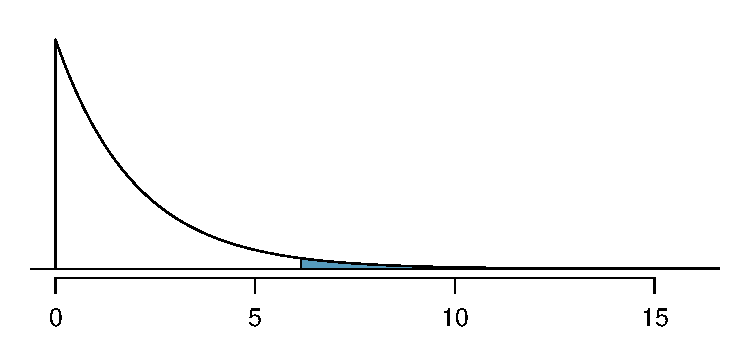
\includegraphics[width=0.7\textwidth]{ch_inference_for_props/figures/googleHTForDiffAlgPerformancePValue/googleHTForDiffAlgPerformancePValue}
\caption{Computing the p-value for the Google hypothesis test.}
\label{googleHTForDiffAlgPerformancePValue}
\end{figure}

\begin{example}{Compute the p-value and draw a conclusion about whether the search algorithms have different performances.}
Looking in Appendix~\ref{chiSquareProbabilityTable} on page~\pageref{chiSquareProbabilityTable}, we examine the row corresponding to 2 degrees of freedom. The test statistic, $\chi^2=6.120$, falls between the fourth and fifth columns, which means the p-value is between 0.02 and 0.05. Because we typically test at a significance level of $\alpha=0.05$ and the p-value is less than 0.05, the null hypothesis is rejected. That is, the data provide convincing evidence that there is some difference in performance among the algorithms.
\index{data!search algorithm|)}
\end{example}

%	Approve	Disapprove
%Obama	56%	41%
%Dem	49%	43%
%Rep	36%	56%
%March 7-11, 2012
%1503 adults

\begin{example}{\index{data!approval ratings|(}Table~\ref{pewResearchPollOnApprovalRatingsForChiSquareSectionExampleAndExercises} summarizes the results of a Pew Research poll.\footnote{See the Pew Research website: \oiRedirect{textbook-obama_and_congress_approval_2012}{www.people-press.org/2012/03/14/romney-leads-gop-contest-trails-in-matchup-with-obama}. The counts in Table~\ref{pewResearchPollOnApprovalRatingsForChiSquareSectionExampleAndExercises} are approximate.} We would like to determine if there are actually differences in the approval ratings of Barack Obama, Democrats in Congress, and Republicans in Congress. What are appropriate hypotheses for such a test?}\label{hypothesisTestSetupForPewResearchPollOnApprovalRatingsForChiSquareSection}
\begin{itemize}
\item[$H_0$:] There is no difference in approval ratings between the three groups.
\item[$H_A$:] There is some difference in approval ratings between the three groups, e.g. perhaps Obama's approval differs from Democrats in Congress.
\end{itemize}
\end{example}

\begin{table}
\centering
\begin{tabular}{ll ccc ll}
& & & \multicolumn{2}{c}{Congress} & \\
\cline{4-5}
 & \hspace{1mm} & Obama & Democrats & Republicans & \hspace{1mm} & Total \\
\hline
Approve				   & & 842    & 736 & 541   & 				& 2119 \\
Disapprove			   & & 616    & 646 & 842   &				& 2104 \\
\hline
Total					   & & 1458    & 1382 & 1383 & 				& 4223 \\
\hline
\end{tabular}
\caption{Pew Research poll results of a March 2012 poll.}
\label{pewResearchPollOnApprovalRatingsForChiSquareSectionExampleAndExercises}
\end{table}

\begin{exercise}
A chi-square test for a two-way table may be used to test the hypotheses in Example~\ref{hypothesisTestSetupForPewResearchPollOnApprovalRatingsForChiSquareSection}. As a first step, compute the expected values for each of the six table cells.\footnote{The expected count for row one / column one is found by multiplying the row one total (2119) and column one total (1458), then dividing by the table total (4223): $\frac{2119\times 1458}{4223} = 731.6$. Similarly for the first column and the second row: $\frac{2104\times 1458}{4223} = 726.4$. Column 2: 693.5 and 688.5. Column 3: 694.0 and 689.0}
% R <- c(2119, 2104); C <- c(1458, 1382, 1383); R*C[1]/sum(C); R*C[2]/sum(C); R*C[3]/sum(C)
\end{exercise}

\begin{exercise}
Compute the chi-square test statistic.\footnote{For each cell, compute $\frac{(\text{obs} - \text{exp})^2}{exp}$. For instance, the first row and first column: $\frac{(842-731.6)^2}{731.6} = 16.7$. Adding the results of each cell gives the chi-square test statistic: {\scriptsize$\chi^2 = 16.7 + \cdots + 34.0 = 106.4$}.}
%R <- c(2119, 2104); C <- c(1458, 1382, 1383); CC <- c(842, 616, 736, 646, 541, 842); EE <- round(c(R*C[1]/sum(C), R*C[2]/sum(C), R*C[3]/sum(C)), 1); (CC-EE)^2/EE; sum((CC-EE)^2/EE)
\end{exercise}

\begin{exercise}
Because there are 2 rows and 3 columns, the degrees of freedom for the test is $df=(2-1)\times (3-1) = 2$. Use $\chi^2=106.4$, $df=2$, and the chi-square table on page~\pageref{chiSquareProbabilityTable} to evaluate whether to reject the null hypothesis.\footnote{The test statistic is larger than the right-most column of the $df=2$ row of the chi-square table, meaning the p-value is less than 0.001. That is, we reject the null hypothesis because the p-value is less than 0.05, and we conclude that Americans' approval has differences among Democrats in Congress, Republicans in Congress, and the president.}
\index{data!approval ratings|)}
\end{exercise}

\CalculatorVideos{the chi-square test for independence}



%__________________
\section[Small sample hypothesis testing for a proportion (special topic)]{Small sample hypothesis testing for a proportion\\(special topic)}
\label{smallSampleHTForProportion}

In this section we develop inferential methods for a single proportion that are appropriate when the sample size is too small to apply the normal model to $\hat{p}$. Just like the methods related to the $t$ distribution, these methods can also be applied to large samples.

\subsection{When the success-failure condition is not met}

\index{data!medical consultant|(}
People providing an organ for donation sometimes seek the help of a special ``medical consultant''. These consultants assist the patient in all aspects of the surgery, with the goal of reducing the possibility of complications during the medical procedure and recovery. Patients might choose a consultant based in part on the historical complication rate of the consultant's clients. One consultant tried to attract patients by noting the average complication rate for liver donor surgeries in the US is about 10\%, but her clients have only had 3 complications in the 62 liver donor surgeries she has facilitated. She claims this is strong evidence that her work meaningfully contributes to reducing complications (and therefore she should be hired!).

\begin{exercise}
We will let $p$ represent the true complication rate for liver donors working with this consultant. Estimate $p$ using the data, and label this value $\hat{p}$.\footnote{The sample proportion: $\hat{p} = 3/62 = 0.048$}
\end{exercise}

\begin{example}{Is it possible to assess the consultant's claim using the data provided?}
No. The claim is that there is a causal connection, but the data are observational. Patients who hire this medical consultant may have lower complication rates for other reasons.

While it is not possible to assess this causal claim, it is still possible to test for an association using these data. For this question we ask, could the low complication rate of $\hat{p} = 0.048$ be due to chance?
\end{example}

\begin{exercise} \label{hypForAssessingConsultantWorkInLiverTransplants}
Write out hypotheses in both plain and statistical language to test for the association between the consultant's work and the true complication rate, $p$, for this consultant's clients.\footnote{$H_0$: There is no association between the consultant's contributions and the clients' complication rate. In statistical language, $p=0.10$. $H_A$: Patients who work with the consultant tend to have a complication rate lower than 10\%, i.e. $p<0.10$.}
\end{exercise}

\begin{example}{In the examples based on large sample theory, we modeled $\hat{p}$ using the normal distribution. Why is this not appropriate here?}
The independence assumption may be reasonable if each of the surgeries is from a different surgical team. However, the success-failure condition is not satisfied. Under the null hypothesis, we would anticipate seeing $62\times 0.10=6.2$ complications, not the 10 required for the normal approximation.
\end{example}

The uncertainty associated with the sample proportion should not be modeled using the normal distribution. However, we would still like to assess the hypotheses from Guided Practice~\ref{hypForAssessingConsultantWorkInLiverTransplants} in absence of the normal framework. To do so, we need to evaluate the possibility of a sample value ($\hat{p}$) this far below the null value, $p_0=0.10$. This possibility is usually measured with a p-value.

The p-value is computed based on the null distribution, which is the distribution of the test statistic if the null hypothesis is true. Supposing the null hypothesis is true, we can compute the p-value by identifying the chance of observing a test statistic that favors the alternative hypothesis at least as strongly as the observed test statistic. This can be done using simulation.


\subsection{Generating the null distribution and p-value by simulation}
\label{generatingTheNullDistributionAndPValueBySimulationForOneProportion}

We want to identify the sampling distribution of the test statistic ($\hat{p}$) if the null hypothesis was true. In other words, we want to see how the sample proportion changes due to chance alone. Then we plan to use this information to decide whether there is enough evidence to reject the null hypothesis.

Under the null hypothesis, 10\% of liver donors have complications during or after surgery. Suppose this rate was really no different for the consultant's clients. If this was the case, we could \emph{simulate} 62 clients to get a sample proportion for the complication rate from the null distribution.

Each client can be simulated using a deck of cards. Take one red card, nine black cards, and mix them up. Then drawing a card is one way of simulating the chance a patient has a complication \emph{if the true complication rate is 10\%} for the data. If we do this 62 times and compute the proportion of patients with complications in the simulation, $\hat{p}_{sim}$, then this sample proportion is exactly a sample from the null distribution.

An undergraduate student was paid \$2 to complete this simulation. There were 5 simulated cases with a complication and 57 simulated cases without a complication, i.e. $\hat{p}_{sim} = 5/62 = 0.081$.

\begin{example}{Is this one simulation enough to determine whether or not we should reject the null hypothesis from Guided Practice~\ref{hypForAssessingConsultantWorkInLiverTransplants}? Explain.}
No. To assess the hypotheses, we need to see a distribution of many $\hat{p}_{sim}$, not just a \emph{single} draw from this sampling distribution.
\end{example}

One simulation isn't enough to get a sense of the null distribution; many simulation studies are needed. Roughly 10,000 seems sufficient. However, paying someone to simulate 10,000 studies by hand is a waste of time and money. Instead, simulations are typically programmed into a computer, which is much more efficient.

Figure~\ref{nullDistForPHatIfLiverTransplantConsultantIsNotHelpful} shows the results of 10,000 simulated studies. The proportions that are equal to or less than $\hat{p}=0.048$ are shaded. The shaded areas represent sample proportions under the null distribution that provide at least as much evidence as $\hat{p}$ favoring the alternative hypothesis. There were 1222 simulated sample proportions with $\hat{p}_{sim} \leq 0.048$. We use these to construct the null distribution's left-tail area and find the p-value:
\begin{align}
\text{left tail }\label{estOfPValueBasedOnSimulatedNullForSingleProportion}
	&= \frac{\text{Number of observed simulations with }\hat{p}_{sim}\leq\text{ 0.048}}{10000}
\end{align}
Of the 10,000 simulated $\hat{p}_{sim}$, 1222 were equal to or smaller than $\hat{p}$. Since the hypothesis test is one-sided, the estimated p-value is equal to this tail area: 0.1222.
\begin{figure}
\centering
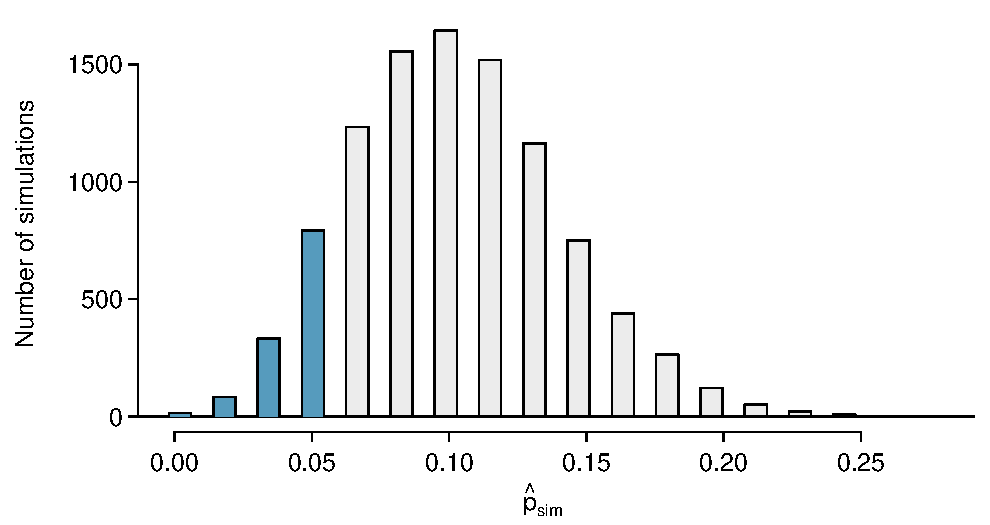
\includegraphics[width=0.9\textwidth]{ch_inference_for_props/figures/nullDistForPHatIfLiverTransplantConsultantIsNotHelpful/nullDistForPHatIfLiverTransplantConsultantIsNotHelpful}
\caption{The null distribution for $\hat{p}$, created from 10,000 simulated studies. The left tail, representing the p-value for the hypothesis test, contains 12.22\% of the simulations.}
\label{nullDistForPHatIfLiverTransplantConsultantIsNotHelpful}
\end{figure}

\begin{exercise} \label{plainLanguageExplanationOfHTConclusionForLiverDonorSurgicalConsultant}
Because the estimated p-value is 0.1222, which is larger than the significance level 0.05, we do not reject the null hypothesis. Explain what this means in plain language in the context of the problem.\footnote{There isn't sufficiently strong evidence to support an association between the consultant's work and fewer surgery complications.}
\index{data!medical consultant|)}
\end{exercise}

\begin{exercise}
Does the conclusion in Guided Practice~\ref{plainLanguageExplanationOfHTConclusionForLiverDonorSurgicalConsultant} imply there is no real association between the surgical consultant's work and the risk of complications? Explain.\footnote{No. It might be that the consultant's work is associated with a reduction but that there isn't enough data to convincingly show this connection.}
\end{exercise}

\begin{termBox}{\tBoxTitle{One-sided hypothesis test for $p$ with a small sample}
The p-value is always derived by analyzing the null distribution of the test statistic. The normal model poorly approximates the null distribution for $\hat{p}$ when the success-failure condition is not satisfied. As a substitute, we can generate the null distribution using simulated sample proportions ($\hat{p}_{sim}$) and use this distribution to compute the tail area, i.e. the p-value.}
\end{termBox}

We continue to use the same rule as before when computing the p-value for a two-sided test: double the single tail area, which remains a reasonable approach even when the sampling distribution is asymmetric. However, this can result in p-values larger than 1 when the point estimate is very near the mean in the null distribution; in such cases, we write that the p-value is 1. Also, very large p-values computed in this way (e.g. 0.85), may also be slightly inflated.

Guided Practice~\ref{plainLanguageExplanationOfHTConclusionForLiverDonorSurgicalConsultant} said the p-value is \emph{estimated}. It is not exact because the simulated null distribution itself is not exact, only a close approximation. However, we can generate an exact null distribution and p-value using the binomial model from Section~\ref{binomialModel}.

\subsection{Generating the exact null distribution and p-value}
\label{exactNullDistributionUsingBinomialModel}

The number of successes in $n$ independent cases can be described using the binomial model, which was introduced in Section~\ref{binomialModel}. Recall that the probability of observing exactly $k$ successes is given by
\begin{align} \label{binomialEquationShownForFindingNullDistributionInSmallSamplePropTest}
P(k\text{ successes}) = {n\choose k} p^{k}(1-p)^{n-k} = \frac{n!}{k!(n-k)!} p^{k}(1-p)^{n-k}
\end{align}
where $p$ is the true probability of success. The expression ${n\choose k}$ is read as \emph{$n$ choose $k$}, and the exclamation points represent factorials. For instance, $3!$ is equal to $3\times 2\times 1=6$, $4!$ is equal to $4\times 3\times 2\times 1 = 24$, and so on (see Section~\ref{binomialModel}).

The tail area of the null distribution is computed by adding up the probability in Equation~\eqref{binomialEquationShownForFindingNullDistributionInSmallSamplePropTest} for each $k$ that provides at least as strong of evidence favoring the alternative hypothesis as the data. If the hypothesis test is one-sided, then the p-value is represented by a single tail area. If the test is two-sided, compute the single tail area and double it to get the p-value, just as we have done in the past.

\begin{example}{Compute the exact p-value to check the consultant's claim that her clients' complication rate is below 10\%.}
Exactly $k=3$ complications were observed in the $n=62$ cases cited by the consultant. Since we are testing against the 10\% national average, our null hypothesis is $p=0.10$. We can compute the p-value by adding up the cases where there are 3 or fewer complications:
\begin{align*}
\text{p-value}
	&= \sum_{j=0}^{3} {n\choose j} p^{j}(1-p)^{n-j} \\
	&= \sum_{j=0}^{3} {62\choose j} 0.1^{j}(1-0.1)^{62-j} \\
	&= {62\choose 0} 0.1^{0}(1-0.1)^{62-0} +
		{62\choose 1} 0.1^{1}(1-0.1)^{62-1} \\
	& \qquad + {62\choose 2} 0.1^{2}(1-0.1)^{62-2} +
		{62\choose 3} 0.1^{3}(1-0.1)^{62-3} \\
	&= 0.0015 + 0.0100 + 0.0340 + 0.0755 \\
	&= 0.1210
\end{align*}
This exact p-value is very close to the p-value based on the simulations (0.1222), and we come to the same conclusion. We do not reject the null hypothesis, and there is not statistically significant evidence to support the association.

If it were plotted, the exact null distribution would look almost identical to the simulated null distribution shown in Figure~\ref{nullDistForPHatIfLiverTransplantConsultantIsNotHelpful} on page~\pageref{nullDistForPHatIfLiverTransplantConsultantIsNotHelpful}.
\end{example}


\subsection{Using simulation for goodness of fit tests}

Simulation methods may also be used to test goodness of fit. In short, we simulate a new sample based on the purported bin probabilities, then compute a chi-square test statistic $X_{sim}^2$. We do this many times (e.g. 10,000 times), and then examine the distribution of these simulated chi-square test statistics. This distribution will be a very precise null distribution for the test statistic $\chi^2$ if the probabilities are accurate, and we can find the upper tail of this null distribution, using a cutoff of the observed test statistic, to calculate the p-value.

\begin{example}{\index{data!racial make-up of jury|(}Section~\ref{oneWayChiSquare} introduced an example where we considered whether jurors were racially representative of the population. Would our findings differ if we used a simulation technique?}
Since the minimum bin count condition was satisfied, the chi-square distribution is an excellent approximation of the null distribution, meaning the results should be very similar. Figure~\ref{jurorChiSquareSimulated} shows the simulated null distribution using 100,000 simulated $X_{sim}^2$ values with an overlaid curve of the chi-square distribution. The distributions are almost identical, and the p-values are essentially indistinguishable: 0.115 for the simulated null distribution and 0.117 for the theoretical null distribution.
\index{data!racial make-up of jury|)}
\end{example}

\begin{figure}[h]
\centering
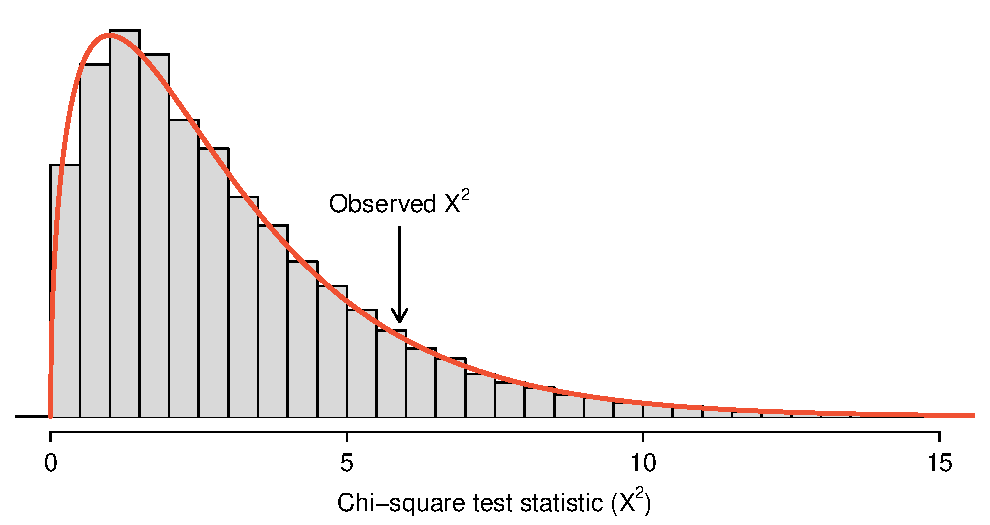
\includegraphics[width=0.9\textwidth]{ch_inference_for_props/figures/jurorChiSquareSimulated/jurorChiSquareSimulated}
\caption{The precise null distribution for the juror example from Section~\ref{oneWayChiSquare} is shown as a histogram of simulated $X_{sim}^2$ statistics, and the theoretical chi-square distribution is also shown.}
\label{jurorChiSquareSimulated}
\end{figure}


%__________________
\section{Randomization test (special topic)}
\label{smallSampleHTForTwoOrMoreProportion}

\Comment{New title for this section.}

\index{data!CPR and blood thinner|(}

Cardiopulmonary resuscitation (CPR) is a procedure commonly used on individuals suffering a heart attack when other emergency resources are not available. This procedure is helpful in maintaining some blood circulation, but the chest compressions involved can also cause internal injuries. Internal bleeding and other injuries complicate additional treatment efforts following arrival at a hospital. For example, blood thinners may be used to release a clot responsible for a heart attack. However, the blood thinner would negatively affect internal bleeding.

We consider an experiment for patients who underwent CPR for a heart attack and were subsequently admitted to a hospital.\footnote{\emph{Efficacy and safety of thrombolytic therapy after initially unsuccessful cardiopulmonary resuscitation: a prospective clinical trial}, by B$\ddot{\text{o}}$ttiger et al., The Lancet, 2001.} These patients were randomly divided into a treatment group where they received a blood thinner or the control group where they did not receive a blood thinner. The outcome variable of interest was whether the patients survived for at least 24 hours.

\begin{example}{What is an appropriate set of hypotheses for this study? Let $p_c$ represent the true survival rate of people who do not receive a blood thinner (corresponding to the control group) and $p_t$ represent the survival rate for people receiving a blood thinner (corresponding to the treatment group).} \label{hypothesesForCPRStudyInSmallSampleSection}
We are interested in whether the blood thinners are helpful or harmful, so a two-sided test is appropriate.
\begin{itemize}
\item[$H_0$:] Blood thinners do not have an overall survival effect, i.e. the survival proportions are the same in each group. $p_t - p_c = 0$.
\item[$H_A$:] Blood thinners do have an impact on survival. $p_t - p_c \neq 0$.
\end{itemize}
\end{example}

\subsection{Large sample framework for a difference in two proportions}

There were 50 patients in the experiment who did not receive the blood thinner and 40 patients who did. The study results are shown in Table~\ref{resultsForCPRStudyInSmallSampleSection}.

\begin{table}[ht]
\centering
\begin{tabular}{lccccc}
\hline
			&& Survived 	& Died 	&& Total \\
\hline
Control		&& 11		& 39		&& 50 \\
Treatment		&& 14		& 26		&& 40 \\
\hline
Total			&& 25		& 65		&& 90 \\
\hline
\end{tabular}
\caption{Results for the CPR study. Patients in the treatment group were given a blood thinner, and patients in the control group were not.}
\label{resultsForCPRStudyInSmallSampleSection}
\end{table}

\begin{exercise}
What is the observed survival rate in the control group? And in the treatment group? Also, provide a point estimate of the difference in survival proportions of the two groups: $\hat{p}_t - \hat{p}_c$.\footnote{Observed control survival rate: $p_c = \frac{11}{50} = 0.22$. Treatment survival rate: $p_t = \frac{14}{40} = 0.35$. Observed difference: $\hat{p}_t - \hat{p}_c = 0.35 - 0.22 = 0.13$.}
\end{exercise}

According to the point estimate, for patients who have undergone CPR outside of the hospital, an additional 13\% survive when they are treated with blood thinners. However, this difference might be explainable by chance. We'd like to investigate this using a large sample framework, but we first need to check the conditions for such an approach.

\begin{example}{Can the point estimate of the difference in survival proportions be adequately modeled using a normal distribution?}
We will assume the patients are independent, which is probably reasonable. The success-failure condition is also satisfied. Since the proportions are equal under the null, we can compute the pooled proportion, $\hat{p} = (11+14)/(50+40) = 0.278$, for checking conditions. We find the expected number of successes (13.9, 11.1) and failures (36.1, 28.9) are above 10. The normal model is reasonable.
\end{example}

While we can apply a normal framework as an approximation to find a p-value, we might keep in mind that the expected number of successes is only 13.9 in one group and 11.1 in the other. Below we conduct an analysis relying on the large sample normal theory. We will follow up with a small sample analysis and compare the results.

\begin{example}{Assess the hypotheses presented in Example~\ref{hypothesesForCPRStudyInSmallSampleSection} using a large sample framework. Use a significance level of $\alpha=0.05$.}
We suppose the null distribution of the sample difference follows a normal distribution with mean 0 (the null value) and a standard deviation equal to the standard error of the estimate. The null hypothesis in this case would be that the two proportions are the same, so we compute the standard error using the pooled proportion:
\begin{align*}
SE = \sqrt{\frac{p(1-p)}{n_t} + \frac{p(1-p)}{n_c}}
	\approx \sqrt{\frac{0.278(1-0.278)}{40} + \frac{0.278(1-0.278)}{50}} = 0.095
\end{align*}
where we have used the pooled estimate $\left( \hat{p} = \frac{11+14}{50 + 40} = 0.278 \right)$ in place of the true proportion, $p$.

The null distribution with mean zero and standard deviation 0.095 is shown in Figure~\ref{pValueCPRStudyLargeSampleAnalysisInSmallSampleSection}. We compute the tail areas to identify the p-value. To do so, we use the Z score of the point estimate:
\begin{align*}
Z = \frac{(\hat{p}_t - \hat{p}_c) - \text{null value}}{SE} = \frac{0.13 - 0}{0.095} = 1.37
\end{align*}
If we look this Z score up in Appendix~\ref{normalProbabilityTable}, we see that the right tail has area 0.0853. The p-value is twice the single tail area: 0.176. This p-value does not provide convincing evidence that the blood thinner helps. Thus, there is insufficient evidence to conclude whether or not the blood thinner helps or hurts. (Remember, we never ``accept'' the null hypothesis -- we can only reject or fail to reject.)
\end{example}
\begin{figure}[ht]
\centering
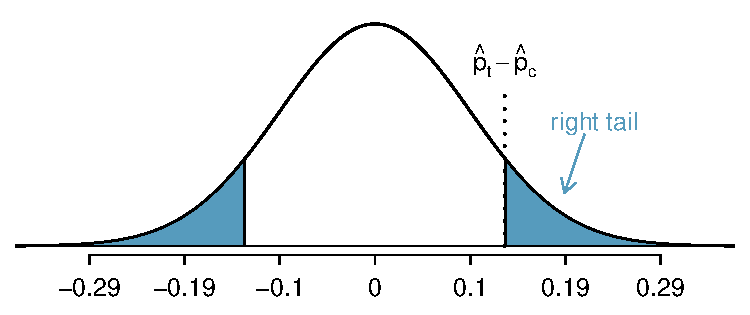
\includegraphics[width=0.75\textwidth]{ch_inference_for_props/figures/pValueCPRStudyLargeSampleAnalysisInSmallSampleSection/pValueCPRStudyLargeSampleAnalysisInSmallSampleSection}
\caption{The null distribution of the point estimate $\hat{p}_t - \hat{p}_c$ under the large sample framework is a normal distribution with mean $0$ and standard deviation equal to the standard error, in this case $SE=0.095$. The p-value is represented by the shaded areas.}
\label{pValueCPRStudyLargeSampleAnalysisInSmallSampleSection}
\end{figure}

The p-value 0.176 relies on the normal approximation. We know that when the samples sizes are large, this approximation is quite good. However, when the sample sizes are relatively small as in this example, the approximation may only be adequate. Next we develop a simulation technique, apply it to these data, and compare our results. In general, the small sample method we develop may be used for any size sample, small or large, and should be considered as more accurate than the corresponding large sample technique.

\subsection{Simulating a difference under the null distribution}

The ideas in this section were first introduced in the optional Section~\vref{caseStudyGenderDiscrimination}. For the interested reader, this earlier section provides a more in-depth discussion.

Suppose the null hypothesis is true. Then the blood thinner has no impact on survival and the 13\% difference was due to chance. In this case, we can simulate \emph{null} differences that are due to chance using a \emph{randomization technique}.\footnote{The test procedure we employ in this section is formally called a \term{permutation test}.} By randomly assigning ``fake treatment'' and ``fake control'' stickers to the patients' files, we could get a new grouping -- one that is completely due to chance. The expected difference between the two proportions under this simulation is zero.

We run this simulation by taking 40 \resp{treatment\_\hspace{0.3mm}fake} and 50 \resp{control\_\hspace{0.3mm}fake} labels and randomly assigning them to the patients. The label counts of 40 and 50 correspond to the number of treatment and control assignments in the actual study. We use a computer program to randomly assign these labels to the patients, and we organize the simulation results into Table~\ref{resultsForCPRStudyInSmallSampleSectionFake1}.
\begin{table}[ht]
\centering
\begin{tabular}{lccccc}
\hline
			&& Survived 	& Died 	&& Total \\
\hline
\resp{control\_\hspace{0.3mm}fake}		&& 15		& 35		&& 50 \\
\resp{treatment\_\hspace{0.3mm}fake}	&& 10		& 30		&& 40 \\
\hline
Total			&& 25		& 65		&& 90 \\
\hline
\end{tabular}
\caption{Simulated results for the CPR study under the null hypothesis. The labels were randomly assigned and are independent of the outcome of the patient.}
\label{resultsForCPRStudyInSmallSampleSectionFake1}
\end{table}

\begin{exercise} \label{exerciseComputingDifferenceForCPRStudyInSmallSampleSectionFake1}
What is the difference in survival rates between the two fake groups in Table~\ref{resultsForCPRStudyInSmallSampleSectionFake1}? How does this compare to the observed 13\% in the real groups?\footnote{The difference is $\hat{p}_{t, fake} - \hat{p}_{c, fake} = \frac{10}{40} - \frac{15}{50} = -0.05$, which is closer to the null value $p_0=0$ than what we observed.}
\end{exercise}

The difference computed in Guided Practice~\ref{exerciseComputingDifferenceForCPRStudyInSmallSampleSectionFake1} represents a draw from the null distribution of the sample differences. Next we generate many more simulated experiments to build up the null distribution, much like we did in Section~\ref{generatingTheNullDistributionAndPValueBySimulationForOneProportion} to build a null distribution for a one sample proportion.

\begin{caution}{Simulation in the two proportion case requires that the null difference is zero}
{The technique described here to simulate a difference from the null distribution relies on an important condition in the null hypothesis: there is no connection between the two variables considered. In some special cases, the null difference might not be zero, and more advanced methods (or a large sample approximation, if appropriate) would be necessary.}
\end{caution}

\subsection{Null distribution for the difference in two proportions}

We build up an approximation to the null distribution by repeatedly creating tables like the one shown in Table~\ref{resultsForCPRStudyInSmallSampleSectionFake1} and computing the sample differences. The null distribution from 10,000 simulations is shown in Figure~\ref{pValueCPRStudySmallSampleAnalysisInSmallSampleSection}.
\begin{figure}
\centering
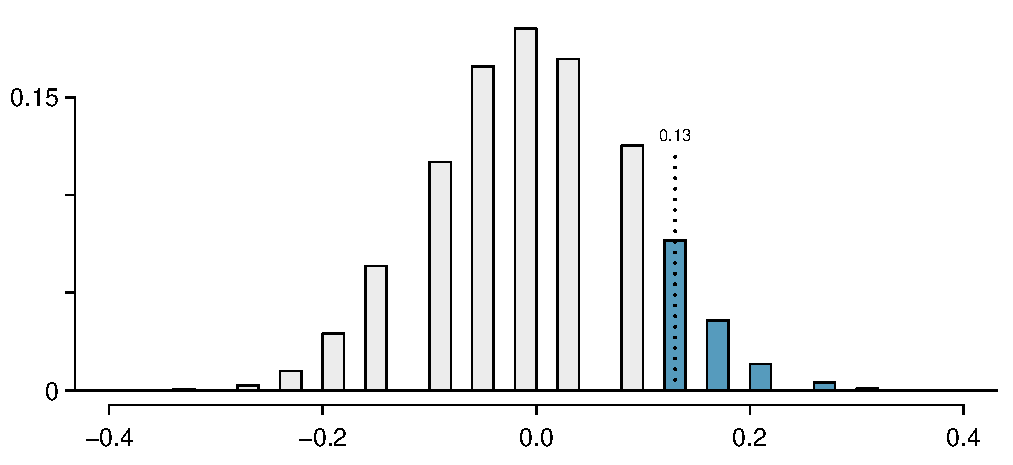
\includegraphics[width=\textwidth]{ch_inference_for_props/figures/pValueCPRStudySmallSampleAnalysisInSmallSampleSection/pValueCPRStudySmallSampleAnalysisInSmallSampleSection}
\caption{An approximation of the null distribution of the point estimate, $\hat{p}_t - \hat{p}_c$. The p-value is twice the right tail area.}
\label{pValueCPRStudySmallSampleAnalysisInSmallSampleSection}
\end{figure}

\begin{example}{Compare Figures~\ref{pValueCPRStudyLargeSampleAnalysisInSmallSampleSection} and~\ref{pValueCPRStudySmallSampleAnalysisInSmallSampleSection}. How are they similar? How are they different?}
The shapes are similar, but the simulated results show that the continuous approximation of the normal distribution is not very good. We might wonder, how close are the p-values?
\end{example}

\begin{exercise} \label{comparisonOfLargeSampleAndSmallSamplePValueInCPRStudy}
The right tail area is about 0.13. (It is only a coincidence that we also have $\hat{p}_t - \hat{p}_c=0.13$.) The p-value is computed by doubling the right tail area: 0.26. How does this value compare with the large sample approximation for the p-value?\footnote{The approximation in this case is fairly poor (p-values: 0.174 vs. 0.26), though we come to the same conclusion. The data do not provide convincing evidence showing the blood thinner helps or hurts patients.}
\index{data!CPR and blood thinner|)}
\end{exercise}

In general, small sample methods produce more accurate results since they rely on fewer assumptions. However, they often require some extra work or simulations. For this reason, many statisticians use small sample methods only when conditions for large sample methods are not satisfied.


\subsection{Randomization for two-way tables and chi-square}

Randomization methods may also be used for the contingency tables. In short, we create a randomized contingency table, then compute a chi-square test statistic $X_{sim}^2$. We repeat this many times using a computer, and then we examine the distribution of these simulated test statistics. This randomization approach is valid for any sized sample, and it will be more accurate for cases where one or more expected bin counts do not meet the minimum threshold of~5. When the minimum threshold is met, the simulated null distribution will very closely resemble the chi-square distribution. As before, we use the upper tail of the null distribution to calculate the p-value.



